\documentclass[conference,a4paper]{IEEEtran}
\IEEEoverridecommandlockouts
\usepackage{cite}
\usepackage{amsmath,amssymb,amsfonts}
\usepackage{graphicx}
\usepackage{booktabs}
\usepackage{array}
\usepackage{xcolor}
\usepackage{url}
\usepackage[hidelinks]{hyperref}
% The rendered PDF carried no document metadata, so a reader's viewer showed the
% file name in place of a title. Author metadata is deliberately left unset: the
% author block on page 1 is the record; duplicating it here adds a second place
% to keep in step.
\hypersetup{
  pdftitle={EdgeCloud: Evidence Budgeting for Edge AI under Degraded Connectivity: A Validation Study of Adaptivity, Admissibility and Adversarial Metadata on Synthetic and Real Disaster Data},
  pdfsubject={Edge AI evidence selection under a shared byte budget and forecast delay},
  pdfkeywords={edge AI, degraded connectivity, multimodal fusion, evidence admissibility,
               conformal prediction, adversarial metadata, disaster data}}
% IEEE conference style sets in Times. Without a Times package the class falls
% back to Computer Modern, which is what this paper shipped in until it was
% checked against the venue template. newtxmath follows amssymb deliberately.
\usepackage{newtxtext,newtxmath}
\usepackage{microtype}
\def\BibTeX{{\rm B\kern-.05em{\sc i\kern-.025em b}\kern-.08em T\kern-.1667em\lower.7ex\hbox{E}\kern-.125emX}}
\newcommand{\authorcheck}[1]{\textcolor{red}{[AUTHOR CHECK: #1]}}
% Master against venue submission. The master carries the complete validated record
% with no page limit. The submission is derived from it by compression for a venue
% page rule. Nothing it omits is lost: every omission is still in the master and
% in the package. Build the master with \submissionfalse.
\newif\ifsubmission
\submissiontrue
\newcommand{\masteronly}[1]{\ifsubmission\else#1\fi}
% Refer to a float that only the master prints. The submission names the package
% instead, so no reference dangles and no number is lost: the prose beside each
% of these carries the values the table tabulates.
\newcommand{\mtab}[2]{\ifsubmission#2\else Table~\ref{#1}\fi}
\newcommand{\mfig}[2]{\ifsubmission#2\else Fig.~\ref{#1}\fi}
% CAMERA-READY: the copyright line and the archival identifier live in camera_ready.tex
% (same directory); fill them there. See that file for the exact format of each.
% camera_ready.tex -- the two camera-ready slots, kept apart from main.tex so they can be
% filled without touching the manuscript source. main.tex reads this file with \input.
%
% 1. Copyright line. Paste the exact string from the acceptance notice between the braces,
%    for example
%      \newcommand{\copyrightline}{978-1-xxxx-xxxx-x/26/\$31.00~\copyright 2026 IEEE}
%    Nothing is printed while it is empty, so the paper never renders a placeholder;
%    scripts/check_submission.py reports the gap instead.
\newcommand{\copyrightline}{}
%
% 2. Archival identifier of the deposited release. The value below is a DUMMY so that the
%    Section XI sentence prints during preparation; replace it with the version DOI that
%    Zenodo (or the chosen repository) mints for release v2.6.18, for example
%      \newcommand{\archivedoi}{10.5281/zenodo.1234567}
%    scripts/check_submission.py FAILS while the dummy is in place, so it cannot reach a
%    submission unnoticed. Set it to {} to print nothing at all.
\newcommand{\archivedoi}{10.5281/zenodo.XXXXXXX}

\makeatletter
\def\@emptyarg{}
\makeatother
\newtheorem{proposition}{Proposition}
\newtheorem{remark}{Remark}

\begin{document}

\title{EdgeCloud: Evidence Budgeting for Edge AI under Degraded Connectivity: A Validation Study of Adaptivity, Admissibility and Adversarial Metadata on Synthetic and Real Disaster Data}

\author{
\IEEEauthorblockN{Sambit Dhar}
\IEEEauthorblockA{Independent Researcher\\Little Rock, United States\\sammy10692@gmail.com}
\and
\IEEEauthorblockN{Arindam Chakraborty}
\IEEEauthorblockA{Independent Researcher\\Texas, United States\\arindamc.81@gmail.com}
\and
\IEEEauthorblockN{Soham Marik}
\IEEEauthorblockA{Independent Researcher\\Texas, United States\\sohammarik63@gmail.com}
\and
\IEEEauthorblockN{Saikat Chakraborty}
\IEEEauthorblockA{Independent Researcher\\Texas, United States\\discoversaikatchakraborty@gmail.com}
\and
\IEEEauthorblockN{Surajit Sinha}
\IEEEauthorblockA{Independent Researcher\\Texas, United States\\surajitsinha1209@gmail.com}
}

\edef\tmpcr{\copyrightline}
\ifx\tmpcr\empty\else
  \IEEEpubid{\makebox[\columnwidth]{\copyrightline\hfill}\hspace{\columnsep}%
             \makebox[\columnwidth]{}}
\fi
\maketitle

\begin{abstract}
Edge AI on degraded field networks must decide what evidence to move and when to stop waiting.
We formulate this as evidence budgeting across concurrent incident windows: a multiple-choice knapsack over a shared byte budget whose latency term prices transfer time together with the
forecast delay of late evidence, so that waiting becomes an explicit decision with a closed-form
threshold. Evidence is fused only when its location, time and hazard tag are admissible; each
decision carries a conformal set and a provenance record. We compare the formulation against
budget-matched simple rules that receive the same information, across nine synthetic conditions at twenty
seeds and a reduced CrisisMMD workload at five. On synthetic data a simple rule is
indistinguishable from the optimizer wherever the budget alone binds and the admissibility filter rather than the optimizer does the work under misaligned reports. A derived delay threshold
cut 95th-percentile latency from 1{,}562.3~s to 25.7~s, with the error difference spanning zero. Forged metadata erases the filter's protection; a reused conformal threshold drops
coverage to 0.745 against a nominal 0.90; measured LTE traces inflate tail latency by up to 8.7 times; an emulated TCP path confirms the latency model's byte term and finds its fixed overhead one round trip short; six
uncoordinated controllers cost the exact knapsack 20.0 errors against 3.9 for a greedy ranking.
On real data the ranking reverses and then proves fragile: across seven event splits the
optimizer leads the fixed rule in 15 of 21 comparisons on the damage label this paper chose, in 14 of 21 once class imbalance is handled and in 11 of 21 on the annotators' own label, where its lead under normal connectivity falls from seven splits to three. A twenty-five-cell diagnostic attributes the text pathway's majority-class output to class imbalance rather than to the reduction; no tested representation clears a bar fixed in advance. On real data the delay threshold keeps a 67- to 74-fold latency reduction in every split while its accuracy gain does not carry over, because that corpus does not decay evidence while a decision waits. What survives is narrow: the formulation earns its place by naming the quantities that matter and supplying a
threshold, never by the solver, which did not reliably beat a greedy alternative; the direction of any real-data comparison is a property of the
label as much as of the method.
\end{abstract}

\begin{IEEEkeywords}
edge AI, degraded connectivity, multimodal fusion, evidence admissibility, conformal prediction, adversarial metadata, disaster data
\end{IEEEkeywords}

\section{Introduction}
A flood, a wildfire or an earthquake produces satellite imagery, field photographs, public reports, weather measurements and infrastructure alarms inside the same hour and almost none of it arrives together. The image waits for the next satellite pass. The network that would carry the raw upload is the network the event has just damaged. A system that waits for everything can be accurate and useless at once, because the decision it supports was needed an hour ago.

This is an edge problem before it is a machine learning problem: which evidence deserves the remaining bandwidth, whether a late observation is worth waiting for and whether a given report belongs to this incident at all. The three decisions are coupled: waiting for an image consumes the time in which other evidence ages; admitting a report from the wrong event corrupts the fusion the budget was spent to enable.

This paper formulates the three decisions jointly and then measures whether the formulation earns its complexity. We treat the coupled problem as evidence budgeting across concurrent incident windows, solve it exactly and compare the resulting policy with the simple rules a practitioner would otherwise deploy. Those rules receive the same information as the optimizer: the same delay forecast, the same incident metadata and the same byte budget. Much of the apparent value of an adaptive method is the value of the information it is fed; the only way to separate the two is to give a simple rule the same information.

The answer is not the one we set out to demonstrate. On the synthetic benchmark at twenty seeds a simple rule derived from the formulation is indistinguishable from the optimizer the formulation justifies wherever the budget alone binds, while the gains elsewhere come from the delay threshold with the admissibility filter rather than from solving the program exactly. On real data the picture changes again, then proves fragile: against that same fixed rule the optimizer leads in 15 of 21 comparisons across seven event splits on the label this paper chose, in 11 of 21 on a label the dataset's own annotators defined, while on the chosen label a single-modality baseline that the formulation would never suggest beats both on errors, for a reason no term in the formulation represents. We report each result, identify its mechanism and draw the consequence.

\ifsubmission
\subsection{What a Reader Gains}
Because the solver is not where the value lies, it is fair to ask what this paper offers beyond ``use
simple rules and test them on your data''. Four things: a closed-form delay
threshold~(\ref{eq:threshold}) that the simple rules do not supply (real-data outcome in Section~\ref{sec:realthreshold}); a recipe for deriving three candidate rules
from the same quantities with an information-matched protocol for choosing among them on
held-out events; evidence about where assumptions fail, namely conformal coverage across
conditions and across events, the byte model against measured payloads, the value
function's blindness to a pathway carrying no signal for this label on this corpus, plus the dependence
of the whole real-data ranking on the labelling (Section~\ref{sec:reallabel}); and two failure
modes for contested deployments: admissibility degrading almost linearly with forging capability
while the exact knapsack loses far more than a greedy rule once controllers cannot
coordinate.

\else
\subsection{What a Reader Gains}
Because the solver is not where the value lies, it is fair to ask what this paper offers beyond ``use
simple rules and test them on your data''. We claim four things. \emph{First}, a
formulation whose first-order condition~(\ref{eq:threshold}) is a closed-form delay
threshold; collapsed to a constant estimated on calibration data, it gives a wait rule
needing no solver, cutting tail latency from 1,562.3~s to 25.7~s, with the error difference
against the policy spanning zero. On real data with a constructed arrival delay it keeps that
reduction in all seven event splits while costing 35.0 errors out of 968, so the
pre-specified test of whether it carries over returns a negative answer
(Section~\ref{sec:realthreshold}). What the threshold buys is lower latency, at a cost that
depends on whether the deployment's evidence goes stale while a decision waits.
\emph{Second}, a recipe for deriving three candidate rules from the same quantities, a
byte-profile fixed rule, the constant threshold and a greedy ranking with a summary floor,
with an information-matched protocol for choosing among them on held-out events; which
rule wins changed between our two workloads while the derivation did not. \emph{Third},
evidence about which assumptions fail: split-conformal coverage fails across operating
conditions and, on real data, within a condition when calibration and test windows come
from different disasters; the byte model is contradicted by measured payloads; the value
function cannot detect a modality carrying no predictive signal for the label under test,
a statement about this pathway on this corpus rather than about the modality; a
twenty-five-cell diagnostic attributes the pathway's behaviour to class imbalance rather than to the
representation; and the direction of the real-data comparison changes with the label, so a
ranking measured on one labelling is not evidence about another
(Section~\ref{sec:reallabel}). \emph{Fourth}, two failure modes for contested deployments:
metadata admissibility degrades almost linearly to nothing as forging capability grows, while the
exact knapsack loses far more than a greedy rule when controllers cannot coordinate. The system is analyst decision support; it does not dispatch, order evacuation or allocate
aid.

\fi
\section{Related Work and Positioning}
\textbf{Multimodal disaster intelligence.} xBD supports building-damage assessment from
satellite imagery~\cite{xbd}; FloodNet and Sen1Floods11 support aerial and radar flood
understanding~\cite{floodnet,sen1floods}, while CrisisMMD pairs text with images from seven
disasters~\cite{crisismmd}, where joint representations improve humanitarian-category
prediction~\cite{ofli2020}. This literature defines what can be learned from disaster data, not what
should be transmitted or withheld when the link degrades.

\textbf{Edge--cloud collaboration.} Edge computing moves computation toward the
data~\cite{shi2016,satya2017}, collaborative inference partitions it by device and network
state~\cite{neurosurgeon} and communication-efficient edge AI treats transmission as a
first-order constraint~\cite{shi2020}. Multimodal systems select what to transmit
adaptively~\cite{dat,cst}, while AVERY adapts a vision--language model's split and
compression to operator intent and bandwidth~\cite{avery}. All of these optimize a single stream or
device; none allocates one budget across concurrent incidents, asks whether a late
observation is worth waiting for or checks that evidence belongs to the incident being
decided.

\textbf{Uncertainty, abstention and trust.} Incomplete-modality learning addresses absent
inputs~\cite{chen2023}, calibration makes probabilities
interpretable~\cite{guo2017}; selective prediction adds a reject
option~\cite{selectivenet}, while split conformal prediction gives marginal coverage under
exchangeability~\cite{sadinle,romano} that does not survive distribution
shift~\cite{ovadia}, which is why we calibrate per condition and measure what reuse costs.

\textbf{What is and is not claimed.} No individual component is new; the combination is.
Patent literature narrows the claim further: disaster-response systems over a
disaster-chain knowledge base~\cite{patent1} and edge--cloud schemes combining evidential
uncertainty, adaptive modality weights and temporal decay~\cite{patent2} predate this work,
so we do not claim the first disaster-specific multimodal edge--cloud framework. The distinctive
feature is methodological: the alternatives receive the same information and the outcome is
reported even when it goes against the proposed method.

\section{System Model and Problem Formulation}
\label{sec:model}
\masteronly{Table~\ref{tab:notation} collects the notation.}

\masteronly{%
\begin{table}[t]
\caption{Notation.}
\label{tab:notation}
\centering\footnotesize
\setlength{\tabcolsep}{3pt}
\begin{tabular}{@{}lp{6.3cm}@{}}
\toprule
Symbol & Definition \\
\midrule
$i$, $s$ & Incident window; slot of $K$ windows sharing budget and link. \\
$m$ & Evidence modality: image, text or sensor. \\
$p_{im}(y)$ & Calibrated class probabilities of the representation sent. \\
$\hat s_i$ & Edge estimate of incident severity. \\
$r_{im}$, $q_{im}$ & Estimated source reliability and input quality, in $[0,1]$. \\
$f_{im}$ & Recency factor, $\exp(-\mathrm{age}_{im}/\tau_m)$. \\
$u_{im}$, $n_{im}$ & Local uncertainty and novelty of item $(i,m)$. \\
$C_{im}(a)$, $L_{im}(a)$ & Serialised byte cost and latency of action $a$. \\
$\hat D_{im}$ & Forecast arrival delay of evidence not yet at the edge. \\
$B$, $R$ & Per-window byte budget and link rate. \\
$\lambda_b$, $\lambda_\ell$ & Byte-cost weight and latency penalty per second. \\
$\hat{\mathcal C}(x)$, $\hat q$ & Conformal set and threshold at error level $\alpha$. \\
\bottomrule
\end{tabular}
\end{table}}%


\subsection{Incident Windows and Admissible Evidence}
An incident window $i$ has a grid cell $c_i$, a decision time $t_i$ and a hazard tag $h_i$. Each evidence item $m$ for that window carries its own cell, observation time and hazard tag; it is admissible only when all three are compatible:
\begin{equation}
\label{eq:adm}
\small
\mathrm{adm}_{im} = \mathbf{1}\big[\|c_{im}-c_i\|_\infty\!\le\! 1\big]\,\mathbf{1}\big[|t_{im}-t_i|\!\le\!\tau^{\mathrm{adm}}_m\big]\,\mathbf{1}\big[h_{im}\!=\!h_i\big].
\end{equation}
An inadmissible item may only be held. In the reference configuration $\tau^{\mathrm{adm}}_m$ is 7,200~s for imagery, 1,800~s for text and 600~s for sensor data; the cell tolerance is one grid step. The rule reads metadata only and never touches labels. Missing evidence is represented explicitly and never imputed.

\subsection{Actions, Objective and Why This Is a Knapsack}
For each admissible item the policy chooses one action $a\in\mathcal A=\{\text{hold},\text{summary},\text{feature},\text{raw}\}$: a summary carries calibrated local probabilities and metadata, a feature carries a quantised embedding and the raw action carries the observation. Holding is not deletion; the item may remain in a local encrypted queue. The $K$ windows of a slot share one budget $KB$ and one link, so the slot policy solves
\begin{align}
\label{eq:knapsack}
\max_{x}\ & \sum_{i\in s}\sum_{m}\sum_{a\in\mathcal A} x_{ima}\Big[v_{im}(a)-\lambda_b\tfrac{C_{im}(a)}{B}-\lambda_\ell L_{im}(a)\Big] \nonumber\\
\text{s.t.}\ & \textstyle\sum_{a} x_{ima}=1\ \ \forall (i,m),\quad \sum_{i,m,a} x_{ima}\,C_{im}(a)\le KB, \nonumber\\
& x_{ima}\in\{0,1\},\quad x_{im,\text{hold}}=1 \text{ if } \mathrm{adm}_{im}=0.
\end{align}
The latency of an action counts its transfer time on the shared link of rate $R$ bytes per second and, for an item not yet at the edge, its forecast arrival delay:
\begin{equation}
\label{eq:latency}
L_{im}(a)=\frac{C_{im}(a)}{R}+\hat D_{im}\,\mathbf 1[(i,m)\ \text{pending}],\ \ L_{im}(\text{hold})=0.
\end{equation}
Holding costs no bytes and no latency. Queueing on the shared link is applied to every method at evaluation time and is not part of the per-item objective. Because each item contributes exactly one action and the slot shares a single budget, (\ref{eq:knapsack}) is a multiple-choice knapsack~\cite{knapsack}.

Evidence value combines estimated severity, reliability, recency, an action-fidelity
multiplier $\phi(a)$, local uncertainty, input quality and novelty against the
admissible evidence. The exact form is the one the reference implementation evaluates:
\begin{equation}
\label{eq:value}
v_{im}(a)=\phi(a)\;\hat s_i\; r_{im}\; f_{im}\,\big(\beta_0+\beta_u u_{im}+\beta_q q_{im}+\beta_n n_{im}\big),
\end{equation}
with $\phi=(0,\,0.34,\,0.64,\,1.0)$ over (hold, summary, feature, raw) and
$\beta_0=0.28$, $\beta_u=0.34$, $\beta_q=0.23$, $\beta_n=0.35$, with $\lambda_b=0.11$ in (\ref{eq:knapsack}). Severity, reliability and recency enter multiplicatively, so any one near zero suppresses the item whatever the others say, while uncertainty, quality and novelty enter as a weighted sum over a positive floor $\beta_0$, so none of those three can suppress an item alone. Recency decays as $f_{im}=\exp(-\mathrm{age}_{im}/\tau_m)$, with $\tau_m$ of 3,600~s for imagery, 900~s for text and 300~s for sensor data. Local uncertainty is $u_{im}=1-\max_y p_{im}(y)$, a proxy for information gain rather than an estimate of it. Novelty is the Jensen--Shannon divergence between the item's local
probabilities and the mean of the local probabilities of the admissible evidence already
present in the window, that mean including the item itself:
\begin{equation}
\label{eq:js}
n_{im}=\mathrm{JS}\!\left(p_{im}\,\Big\|\,\bar p_i\right),\qquad
\bar p_i=\frac{1}{|P_i|}\sum_{m'\in P_i} p_{im'},
\end{equation}
where $P_i$ is the set of admissible modalities whose local output has arrived. For an image
that has not yet arrived no local output exists, so $u_{im}$ is set to $1-\max_y \bar p_i(y)$ over the
evidence already present, $q_{im}$ takes the prior mean $5/7$ and $n_{im}=0$.

These coefficients are configuration rather than fitted quantities, set by hand as Section~\ref{sec:limits} records. They are stated because the factor list alone is not enough to reproduce the policy. Disagreement does not enter (\ref{eq:value}): it is a separate per-window quantity, the largest Jensen--Shannon divergence between any two selected modalities, zero when fewer than two are selected; it is what the conflict rule of Section~\ref{sec:queue} thresholds. The action-fidelity multiplier is the whole of the action's effect on value.

\subsection{The Wait-or-Act Decision}
\label{sec:wait}
Because a pending item carries its forecast delay inside $L_{im}(a)$, waiting is not a heuristic bolted on beside the allocator. When the slot budget is not binding, (\ref{eq:knapsack}) separates by item and a non-hold action $a$ is selected for a pending item only when its net utility is positive:
\begin{equation}
v_{im}(a)-\lambda_b\frac{C_{im}(a)}{B}-\lambda_\ell\Big(\frac{C_{im}(a)}{R}+\hat D_{im}\Big)>0.
\end{equation}
Rearranging gives a threshold on the forecast delay,
\begin{equation}
\label{eq:threshold}
\hat D_{im}<T_{im}(a)\ \equiv\ \frac{v_{im}(a)-\lambda_b\,C_{im}(a)/B}{\lambda_\ell}-\frac{C_{im}(a)}{R},
\end{equation}
and the policy waits for the item when $\max_{a\neq\text{hold}}T_{im}(a)>\hat D_{im}$. The threshold rises with severity, reliability and the uncertainty of the evidence already in hand (all of which enter through $v_{im}(a)$) and falls with byte cost and with $\lambda_\ell$. The coefficient $\lambda_\ell$ therefore states how many units of evidence value one second of delay costs and sweeping it traces an accuracy--latency frontier. When the budget binds, the knapsack trades waiting against other windows' needs. A decision that waits also ages the evidence it holds, which fusion accounts for through $f_{im}$.

Collapsing the threshold to a constant gives a rule that needs no optimizer: for the image-summary action, take
\begin{equation}
\label{eq:tstar}
T^\ast=\operatorname{median}\{\,T_{im}(\text{summary}): (i,m)\in\mathcal W_{\mathrm{cal}}\,\},
\end{equation}
over calibration windows $\mathcal W_{\mathrm{cal}}$ whose image is pending, fix $T^\ast$ before testing and wait for a late image only when $\hat D_{im}<T^\ast$. Across the five package seeds $T^\ast$ was 196--219~s. Section~\ref{sec:delay} compares that rule with the policy it came from.

\subsection{Properties}
\begin{proposition}[Feasibility and exactness]\label{prop:exact}
Round each byte cost up to a multiple of $\delta=KB/2000$ and solve (\ref{eq:knapsack}) by dynamic programming over the rounded budget~\cite{knapsack}. Every returned allocation satisfies the true budget, because rounding up can only overstate cost; the returned allocation is optimal for the rounded problem. Each of the $3K$ items loses at most $\delta$ bytes of capacity to rounding, so the allocation is also optimal for the original problem whenever that problem has an optimum leaving at least $3K\delta$ bytes unused, which is 0.9\% of the slot budget at $K=6$.
\end{proposition}

\begin{proposition}[Coverage within a condition]\label{prop:coverage}
If calibration and test windows are exchangeable within an operating condition, the conformal set of (\ref{eq:conformal}) contains the true class with probability at least $1-\alpha$ for that condition, where $\alpha$ is the conformal error level~\cite{sadinle}. No guarantee is claimed across conditions; Section~\ref{sec:coverage} measures what is lost when one threshold is reused and Section~\ref{sec:real} shows the premise failing within a condition on real data, where calibration and test windows come from different disasters.
\end{proposition}

\begin{remark}[Severity cannot confirm]
Severity appears only in the rule that routes a case to human review, never in the rule that assigns a confirmed status, so a severe but ambiguous case can be escalated but never confirmed. Severity is the quantity most likely to be correlated with operator anxiety and least likely to be well estimated.
\end{remark}

\section{Method}
Each edge node runs a lightweight model producing class probabilities calibrated by temperature scaling on calibration events~\cite{guo2017}. The cloud holds one model per representation: a feature model trained only on the transmitted quantised embedding and a raw model trained on the full observation. No representation is scored with information it did not carry. Severity is estimated at the edge from the local probabilities of the admissible evidence already present.

For each window the 64 action combinations over three modalities are enumerated with their utilities and byte costs; the dynamic program processes windows in turn with a back-pointer at every rounded budget level and the allocation is recovered by backtracking, at $O(K\cdot 64\cdot 2000)$ operations per slot. All-hold is permitted only for a window with no admissible evidence.

Selected posteriors are combined by a weighted logarithmic opinion pool~\cite{heskes} over normalised weights,
\begin{equation}
\label{eq:pool}
p_i(y)\ \propto\ \prod_{m\in S_i} p_{im}(y)^{w_{im}},\qquad \sum_{m\in S_i} w_{im}=1,
\end{equation}
where $S_i$ is the set of modalities transmitted for window $i$. Because the weights are normalised, adding a corroborating modality changes the posterior through its content and not through the number of sources; corroboration is handled in the status rule instead. Before that normalisation the weight is $W_m q_{im} r_{im} f_{im}$, with $W$ of 0.40 for imagery, 0.35 for text and 0.25 for sensor data. If a decision waits for an image, the evidence it holds ages by the waiting time before fusion.

The fused posterior becomes a split-conformal set using the least-ambiguous set-valued classifier score~\cite{sadinle}:
\begin{equation}
\label{eq:conformal}
\hat{\mathcal C}(x)=\{\,y: p_i(y)\ge\hat q\,\},
\end{equation}
where $\hat q$ is the $\lfloor \alpha(n_{\mathrm{cal}}+1)\rfloor$-th smallest true-class probability $p_j(y_j)$ over the $n_{\mathrm{cal}}$ calibration windows $j$ processed under the same operating condition. When $\hat q$ exceeds 0.5 a set can contain at most one class, because two classes whose probabilities both reach the threshold would sum to more than one, so a non-singleton set is empty: no class reaches the threshold and the method abstains. \mtab{tab:status}{A table in the package} maps the set, the fused confidence and the conflict indicator to an operational status: a singleton set with confidence at least 0.90 from at least two modalities is confirmed, any other singleton likely; a non-singleton set is insufficient evidence; a maximum pairwise Jensen--Shannon divergence of at least 0.15 marks conflict; an estimated severity of at least 0.70 alongside either of those two escalates to human review.

\masteronly{%
\begin{table}[t]
\caption{Operational statuses. Thresholds are configuration parameters, not learned quantities.}
\label{tab:status}
\centering\footnotesize
\begin{tabular}{@{}p{1.6cm}p{2.9cm}p{3.0cm}@{}}
\toprule
Status & Rule & System behaviour \\
\midrule
Human review required & $\hat s\ge0.70$ and (set size $\ne1$ or conflict) & Escalate with reason codes. \\
Insufficient evidence & Set size $\ne1$ & Withhold a categorical recommendation; queue to seek evidence. \\
Conflicting & Maximum pairwise JS divergence $\ge0.15$ & Preserve competing evidence; queue. \\
Confirmed & Singleton set with confidence $\ge0.90$ from at least two modalities & Place high in the analyst queue; no autonomous dispatch. \\
Likely & Singleton set otherwise & Monitor; present uncertainty. \\
\bottomrule
\end{tabular}
\end{table}}%


Every decision is written to a provenance envelope recording the window, event and slot identifiers, each item's metadata, admissibility, action, bytes, reason code and source digest, the model, policy and calibration versions, the probabilities, the conformal set, the status and the rule that fired, plus a digest of the envelope itself. Completeness is computed by checking those fields for every selected item. A digest links a decision to retained source data; it does not establish that the source is true.

\section{Reference Implementation and Evaluation Protocol}
\subsection{Implementation and Integrity Tests}
The implementation is a set of deterministic Python modules called by the accompanying notebook. A configuration file fixes seeds, event splits, conditions, the byte model, recency scales, admissibility tolerances, policy coefficients and thresholds. Five integrity properties are tested rather than assumed: the transmission policy is unchanged when test labels and generating severities are permuted; budget-compliant methods never exceed a slot budget; the admissibility rule never rejects aligned evidence; the fixed rule with admissibility never sends an inadmissible item; and the derived wait threshold is computed from calibration events only, is unchanged under label permutation and causes the rule to wait exactly for images whose forecast delay lies below it.

\subsection{Workload and Network Model}
\label{sec:workload}
A synthetic generator creates three classes and image, text and sensor feature vectors for 12 event identities with 180 windows each, every event carrying a grid location and a hazard tag; edge models see a prefix of each vector, the raw cloud model all of it and the feature model a quantised principal-component embedding. Byte sizes are assumptions: summaries 184--224 bytes, features 768--2,048 bytes, raw images 220--620~kB, raw text 350--1,800 bytes and raw sensor records 220--900 bytes. Section~\ref{sec:real} measures these against real payloads and finds them wrong. Events D00--D05 train the models, D06--D07 calibrate them and D08--D11 are held out for testing, so no test event contributes to any fitted quantity. The severity estimator's mean training $R^2$ across seeds was 0.10, which is weak and is treated as such throughout.

Connectivity is modelled, the emulator check of Section~\ref{sec:exploratory} being the only packet-level test. Windows form slots of $K=6$ by decision time within an event. The windows in a slot share a budget of $KB$ bytes and one link, served in order of estimated severity, so queueing delay applies to every method including the unconstrained reference. In the delayed-imagery condition 70\% of images arrive after a log-normal delay with a 900~s median and the policy sees only a forecast with multiplicative log-normal error ($\sigma=0.4$). There is no MAC layer, routing or contention model in the base configuration; what it captures is the coupling between byte volume, a shared serving order and decision latency. Section~\ref{sec:link} relaxes two of those assumptions by adding loss with retransmission and capacity replayed from third-party measurements.

\subsection{Questions, Methods and Conditions}
The confirmatory evaluation (Section~\ref{sec:results}) asks whether adaptive selection beats simple budget-compliant rules when bandwidth is the only constraint, how the wait-or-act decision trades errors against latency, whether admissibility keeps misaligned evidence out of fusion, how calibration and the review queue behave across conditions and whether exact optimization beats simple allocation when the shared budget binds. The waiting and admissibility questions are each answered against a rule that receives the same information as the optimizer. Questions asked after those answers were in hand (metadata forgery, link realism, uncoordinated controllers and a measured workload) are reported as exploratory in Sections~\ref{sec:exploratory} and~\ref{sec:real}.

Each seed provides 720 held-out test windows. We report the mean of twenty seeds with two-sided 95\% $t$ intervals and paired seed-level differences; these describe benchmark variability rather than population inference. The first five seeds reproduce the package's published means exactly, the run stopping on any mismatch. Three of the eight paired error comparisons still include zero at twenty seeds, so we treat those three as inconclusive rather than as equivalence. The main protocol was not pre-registered. The information-matched baselines and the review-rule sensitivity analysis were added after an internal audit of the prototype; the wait threshold was fixed on calibration events and the review settings were left unchanged. The two contested-budget experiments of Section~\ref{sec:contested} were pre-registered with frozen protocol files whose SHA-256 digests are checked at run time. \ifsubmission The package lists every method with its description and every condition with its exact manipulation.\else Tables~\ref{tab:methods} and~\ref{tab:conditions} list the methods and conditions.\fi

\masteronly{%
\begin{table}[t]
\caption{Methods compared. The derived threshold and the fixed rule with admissibility exist to give a simple rule the same information the optimizer receives.}
\label{tab:methods}
\centering\footnotesize
\setlength{\tabcolsep}{3pt}\begin{tabular}{@{}p{1.9cm}p{4.1cm}p{1.4cm}@{}}
\toprule
Method & Description & Budget \\
\midrule
Image only / text only & Local summary of one modality. & Compliant \\
Transmit all & Raw evidence for every available modality. & Reference; ignores budget \\
Confidence gate & Raw when local confidence $<0.72$, else summary; downgraded until the window fits. & Compliant \\
Fixed compression & Feature for every available modality. & Compliant \\
Fixed rule & Image summary, raw text, raw sensor. & Compliant \\
Random within budget & Uniform choice among feasible action combinations. & Compliant \\
Wait if uncertain & Fixed rule, but wait for a late image only if text--sensor confidence $<0.90$. & Compliant \\
Derived threshold & Fixed rule, but wait only if forecast delay $<T^\ast$ of (\ref{eq:tstar}). & Compliant \\
Fixed rule + admissibility & Fixed rule with the filter of (\ref{eq:adm}). & Compliant \\
Proposed & Shared-budget knapsack (\ref{eq:knapsack}) with admissibility and forecast delay. & Compliant \\
\bottomrule
\end{tabular}
\end{table}}%


\masteronly{%
\begin{table}[t]
\caption{Operating conditions.}
\label{tab:conditions}
\centering\footnotesize
\begin{tabular}{@{}p{2.3cm}p{5.2cm}@{}}
\toprule
Condition & Manipulation \\
\midrule
Normal & 10~Mbps link; 360~kB per-window budget. \\
Low bandwidth & 256~kbps; 4,000-byte per-window budget. \\
Delayed imagery & 2~Mbps; 70\% of images late (median 900~s); forecast only. \\
Intermittent outage & 512~kbps; 12~s interruption for 35\% of windows. \\
Image / text missing & Remove all images / all text. \\
Noisy text & Soften text probabilities for 35\% of windows; imperfect quality indicator. \\
Contradictory evidence & Point text toward a wrong class for 35\% of windows; imperfect reliability indicator. \\
Misaligned evidence & Replace 30\% of text items with reports from other events; 25\% of those carry compatible metadata. \\
\bottomrule
\end{tabular}
\end{table}}%


Among the general baselines only the proposed method applies the admissibility rule, so the whole-system comparison under misaligned evidence does not isolate it; the fixed rule with admissibility and the corresponding ablation do. Budget-compliant methods never exceeded a slot budget in any run and provenance completeness was 100\% for every method and condition.

\section{Confirmatory Results on the Synthetic Benchmark}
\label{sec:results}
\subsection{When Bandwidth Is the Only Constraint, a Fixed Rule Is Enough}
Table~\ref{tab:lowbw} gives the low-bandwidth condition. Among budget-compliant methods the policy and the fixed rule made statistically indistinguishable numbers of errors, a paired difference of $-0.8$ $[-1.7, 0.2]$. At five seeds the fixed rule held a nominal $+0.2$; at twenty the sign reverses and the interval still spans zero, so neither method is ahead. The policy spent 1,745 more bytes per window $[1{,}732, 1{,}757]$ and added 0.33~s to tail latency $[0.330, 0.334]$, buying image features that do not change the decision under this byte model. Transmit-all reaches 84.6~s at the tail because six windows share one link. The same pattern holds wherever the byte budget is the only binding constraint: under normal connectivity, under an intermittent outage and with imagery missing, the paired difference spans zero in each case. It does not hold once the evidence itself degrades. With text missing the policy is ahead by 2.75 errors $[1.03, 4.47]$, under noisy text by 1.30 $[0.13, 2.47]$ and under contradictory evidence by 2.50 $[0.80, 4.20]$, all three excluding zero at twenty seeds where five seeds could not separate them (\mtab{tab:allcond}{every condition is tabulated in the package}). When no decision involves waiting, admissibility or degraded evidence, the optimizer adds cost rather than value. Section~\ref{sec:link} shows that the cost grows once the link is modelled with loss and measured variability.

\begin{table}[t]
\caption{Low bandwidth (256~kbps, 4,000 bytes per window). Errors out of 720, mean of twenty seeds with 95\% intervals. Every column, the queue share included, comes from the same twenty-seed run. *Ignores the budget.}
\label{tab:lowbw}
\centering\scriptsize\setlength{\tabcolsep}{3pt}
\begin{tabular}{@{}lrrrr@{}}
\toprule
Method & Errors [95\% CI] & Bytes & p95 s & Queue \\
\midrule
Image only & 71.5 [59.1, 83.9] & 224 & 0.27 & 7\% \\
Text only & 75.7 [63.9, 87.4] & 196 & 0.26 & 6\% \\
Transmit all* & 4.3 [2.9, 5.7] & 423,502 & 84.64 & 33\% \\
Confidence gate & 7.0 [5.0, 9.0] & 1,063 & 0.47 & 30\% \\
Fixed compression & 4.4 [3.0, 5.8] & 3,840 & 0.95 & 32\% \\
Fixed rule & 5.2 [3.6, 6.7] & 1,860 & 0.59 & 34\% \\
Random within budget & 22.6 [18.5, 26.6] & 1,695 & 0.60 & 27\% \\
Proposed & 4.4 [3.2, 5.6] & 3,604 & 0.92 & 32\% \\
\bottomrule
\end{tabular}
\end{table}

\subsection{Waiting for Late Evidence: The Threshold Matters, the Solver Does Not}
\label{sec:delay}
Table~\ref{tab:delay} gives the delayed-imagery condition. Methods that always wait paid a median latency near 682.8~s. The policy sent 37\% of images, those with short forecast delays or uncertain partial evidence as (\ref{eq:threshold}) predicts, holding its median latency at 0.19~s. Against the wait-if-uncertain rule, which ignores the forecast, it changed tail latency by $-1{,}197$~s $[-1{,}250, -1{,}145]$. Removing the latency penalty cost $9.1$ errors $[5.6, 12.5]$ and made it wait for every image, which confirms that the term is doing the work (\mtab{tab:ablation}{every ablation is tabulated in the package}).

\begin{table}[t]
\caption{Delayed imagery. Errors out of 720 with 95\% intervals, mean of twenty seeds; median and 95th-percentile modelled latency; share of images sent. *Ignores the budget.}
\label{tab:delay}
\centering\scriptsize\setlength{\tabcolsep}{3pt}
\begin{tabular}{@{}lrrrr@{}}
\toprule
Method & Errors [95\% CI] & Median s & p95 s & Image sent \\
\midrule
Image only & 71.5 [59.1, 83.9] & 682.80 & 1,864.4 & 100\% \\
Text only & 75.7 [63.9, 87.4] & 0.15 & 0.15 & 0\% \\
Transmit all* & 19.2 [15.5, 23.0] & 688.69 & 1,869.5 & 100\% \\
Confidence gate & 25.6 [21.1, 30.0] & 682.81 & 1,864.4 & 100\% \\
Fixed compression & 18.9 [14.9, 23.0] & 682.84 & 1,864.4 & 100\% \\
Fixed rule & 23.4 [18.7, 28.1] & 682.82 & 1,864.4 & 100\% \\
Random within budget & 32.1 [28.1, 36.2] & 39.69 & 1,664.7 & 68\% \\
Wait if uncertain & 16.0 [12.3, 19.7] & 42.56 & 1,562.3 & 53\% \\
Derived threshold $T^\ast$ & 10.8 [8.6, 13.0] & 0.18 & 25.7 & 31\% \\
Proposed, $\lambda_\ell=0.0004$ & 10.2 [8.3, 12.0] & 0.19 & 364.9 & 37\% \\
\bottomrule
\end{tabular}
\end{table}

The latency reduction does not require the optimizer. The derived-threshold rule sends the fixed rule's image summary whenever the forecast delay falls below the calibration-derived constant $T^\ast$. It sent 31\% of images and made 10.8 errors at 25.7~s tail latency. Relative to it the policy changed errors by $-0.7$ $[-1.5, 0.2]$, tail latency by $+339.2$~s $[314.4, 363.9]$ and bytes by $+688$ $[670, 706]$. The error interval includes zero at twenty seeds as it did at five, which is the evidence for the claim in this subsection title. The policy's longer tail comes from per-window adaptivity: it waited more than 300~s for 5.9\% of windows against 0.5\% for the constant rule, when uncertain partial evidence raised the value of a late image. Fig.~\ref{fig:frontier} shows that the constant-threshold frontier lies on or slightly below the policy's throughout.

\begin{figure}[t]
\centering
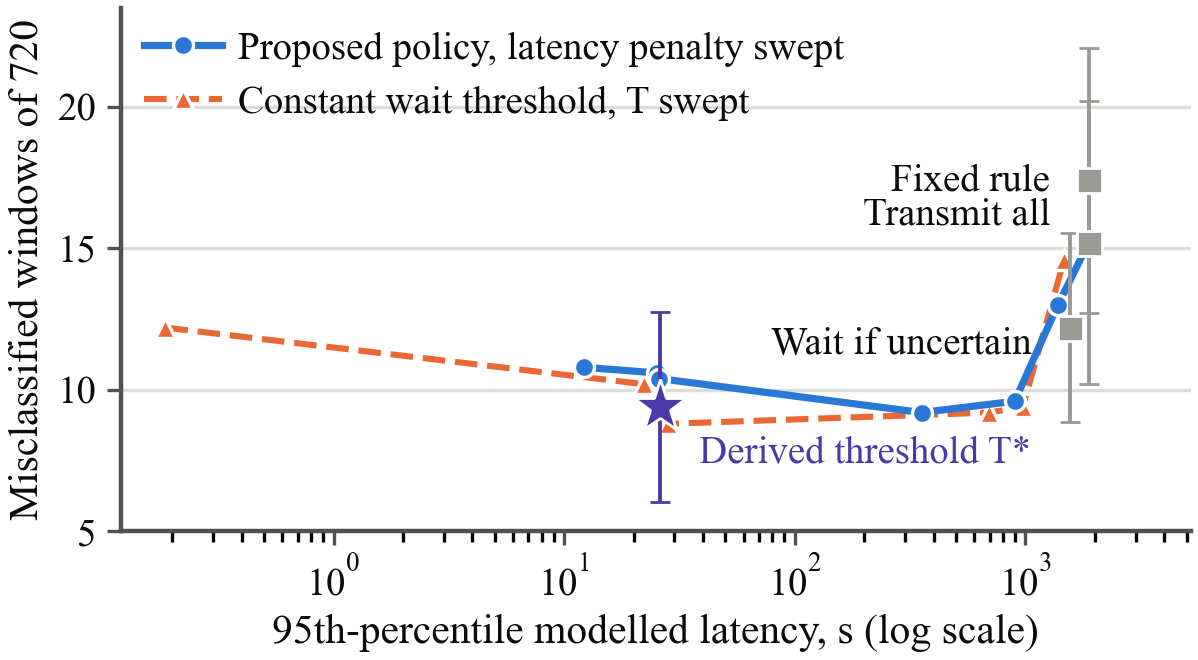
\includegraphics[width=\columnwidth]{fig_delay_frontier.png}
\caption{Delayed imagery: errors against 95th-percentile modelled latency. The solid line traces the policy across latency-penalty values; the dashed line traces the constant-threshold rule across $T$. The star marks $T^\ast$ derived from calibration events, not selected on test data. The sweep is the five-seed package run, not the twenty-seed rerun of Table~\ref{tab:delay}.}
\label{fig:frontier}
\end{figure}


The accuracy comparison carries a caveat that changes the conclusion. The policy changed errors by $-13.3$ $[-17.3, -9.2]$ against the fixed rule and by $-5.9$ $[-8.5, -3.2]$ against wait-if-uncertain. Those gains exist because the benchmark decays the weight of text and sensor evidence while a decision waits. With that decay removed, the forecast-ignoring baselines improve by 10.6 to 18.3 errors while the two forecast-using rules change by at most 0.5, so the ordering reverses: the fixed rule reaches 5.2 errors and wait-if-uncertain 5.4 against 9.7 for the policy and 10.7 for the derived threshold (sensitivity rows of the twenty-seed ablation results). Without staleness, both forecast-using rules trade 4.5 to 5.6 errors for their latency reduction. Whether acting early also improves accuracy therefore depends on how fast real evidence goes stale, which this benchmark assumes rather than measures; Section~\ref{sec:realthreshold} tests that on a corpus with no decay.

\subsection{Admissibility, Not Optimization, Keeps Foreign Reports Out}
\label{sec:adm}
When 30\% of text items came from other events, methods without the admissibility rule fused all of them. The proposed method fused 24\% of misaligned items, exactly those whose metadata had been made compatible and rejected no aligned item. The complete system made 13.9 errors against 35.0 for the fixed rule without admissibility, a paired difference of $-21.1$ $[-26.2, -15.9]$. The fixed rule with the same filter made 15.3 errors; relative to it the proposed method changed errors by $-1.5$ $[-2.7, -0.3]$. The filter accounts for almost all of the gain and at twenty seeds the residual advantage of the optimizer over the filtered simple rule is small while its interval no longer spans zero. Within the proposed system, disabling admissibility added $+16.2$ errors $[11.1, 21.3]$; at five seeds that interval included zero, so the filter's own effect is now estimated precisely enough to read.

This test favours the filter by construction. Aligned evidence shares the window's cell and hazard tag exactly and is at most 60~s old, far inside the tolerances, while misaligned reports that were not spoofed carry the coordinates of another event on a $400\times400$ grid. Zero false rejections follow from the generator, not from the rule's robustness. Real metadata carries positional error, clock skew and missing geotags, none of which is represented here.

\subsection{Conformal Coverage Does Not Survive a Change of Condition}
\label{sec:coverage}
Calibrating per condition kept empirical coverage between 0.889 and 0.899 at twenty seeds against a nominal 0.90; the shortfall is consistent with having only two calibration events. Reusing the normal-condition threshold is where the trouble starts. Coverage falls to 0.794 under contradictory evidence and to 0.745 with images missing, a loss of 13.8 percentage points in the condition where an operator is most likely to rely on the interval; these reuse figures are the five-seed package sweep, which has no twenty-seed rerun. Proposition~\ref{prop:coverage} should not be stretched across conditions: a deployment that calibrates once at commissioning will be miscalibrated exactly when the network degrades. Section~\ref{sec:real} shows that per-condition recalibration is necessary but not sufficient, because on real data the guarantee also fails across events.

\subsection{The Review Queue Is the Real Operational Cost}
\label{sec:queue}
Under low bandwidth about 30\% of windows entered the combined abstention and review queue, roughly 61 queued windows per caught error; under contradictory evidence 53\% did. The queue figures in this subsection come from the package's five-seed sensitivity run rather than the twenty seeds of Table~\ref{tab:lowbw} (the full table, for all nine conditions, is in the package). Under low bandwidth 98\% of queued windows were correctly classified, so almost all reviewer effort confirmed a decision the system had already got right. Conformal abstention alone queued about 10\% of windows and still caught every error; the pre-specified conflict rule nearly tripled the queue without catching an additional one. Across conditions the conflict rule added 11 to 43 percentage points of queue load for between zero and two additional caught errors per 720 windows. We keep the pre-specified settings rather than tune after the fact; the implication is that the conflict threshold is a staffing decision and should be set from reviewer capacity. The severity-based escalation rule was nearly inert, firing on 0.07\% of windows against the 28\% the generating severity would have escalated, because the severity estimator is weak.

\subsection{When the Shared Budget Binds (Pre-registered)}
\label{sec:contested}
None of the conditions above makes the shared budget bind, which is the only regime in which the knapsack can differ from a per-window rule. At the reference difficulty it could not have mattered: on calibration events, sending only summaries erred on 0.56\% of windows against 0.44\% for the unconstrained fixed rule. We therefore froze a protocol before running the proposed method on a harder condition, with the protocol file and its SHA-256 digest inside the package. Observation noise was scaled by 1.75, the smallest value in a pre-specified grid at which summaries alone err on at least 8\% of calibration windows. Models were retrained at that difficulty, the link runs at 256~kbps with $K=6$ and per-window budgets range from 700 to 1,900 bytes, with ten seeds. The pre-specified competitor is a shared-budget greedy rule that starts from summaries and upgrades items across the slot in order of local uncertainty; a greedy heuristic on the proposed utility isolates the exact solver. A difference counts only if its paired $t$-test survives Holm adjustment~\cite{holm} across the five budgets at 0.05.

\masteronly{%
\begin{table}[t]
\caption{Contested shared budget (noise scale 1.75, ten seeds): errors out of 720 by per-window byte budget $B$. *Ignores the budget; shown as a ceiling.}
\label{tab:contested}
\centering\scriptsize\setlength{\tabcolsep}{3pt}
\begin{tabular}{@{}p{2.3cm}rrrrr@{}}
\toprule
Method & 700 & 900 & 1,200 & 1,500 & 1,900 \\
\midrule
Summaries only & 78.6 & 78.7 & 78.6 & 78.6 & 78.8 \\
Fixed rule, per window & 78.6 & 75.1 & 68.9 & 65.6 & 64.0 \\
Confidence gate & 78.6 & 76.0 & 70.0 & 66.3 & 64.7 \\
Random within budget & 140.4 & 141.3 & 127.1 & 121.1 & 109.2 \\
Greedy by uncertainty & 76.0 & 71.2 & 68.9 & 63.3 & 61.9 \\
Greedy, proposed utility & 96.4 & 72.3 & 64.6 & 60.7 & 57.2 \\
Proposed (exact knapsack) & 96.8 & 72.6 & 64.9 & 59.7 & 57.1 \\
Fixed rule, ignores budget* & 57.6 & 57.5 & 57.7 & 57.5 & 57.4 \\
\bottomrule
\end{tabular}
\end{table}}%


The optimizer did not beat the pre-specified competitor at any budget (\mtab{tab:contested}{the full grid is in the package}, Fig.~\ref{fig:contested}). At 700 bytes it was worse by $+20.8$ errors $[15.4, 26.2]$ with Holm $p<0.001$. At the three largest budgets it led nominally by $-4.0$, $-3.6$ and $-4.8$ errors and none survived adjustment (Holm $p$ 0.075 to 0.219). The exact solver matched a greedy solver on the same utility to within one error at every budget. One of those five solver-versus-greedy differences, at $B=1{,}500$ bytes, survived Holm adjustment in the solver's favour ($p=0.042$); it is 1.0 error in 720 (0.14\% of windows). We do not regard that as a benefit worth an exact solver, but the pre-specified decision rule was met once and it would be wrong to say the solver never beat greedy.

\begin{figure}[t]
\centering
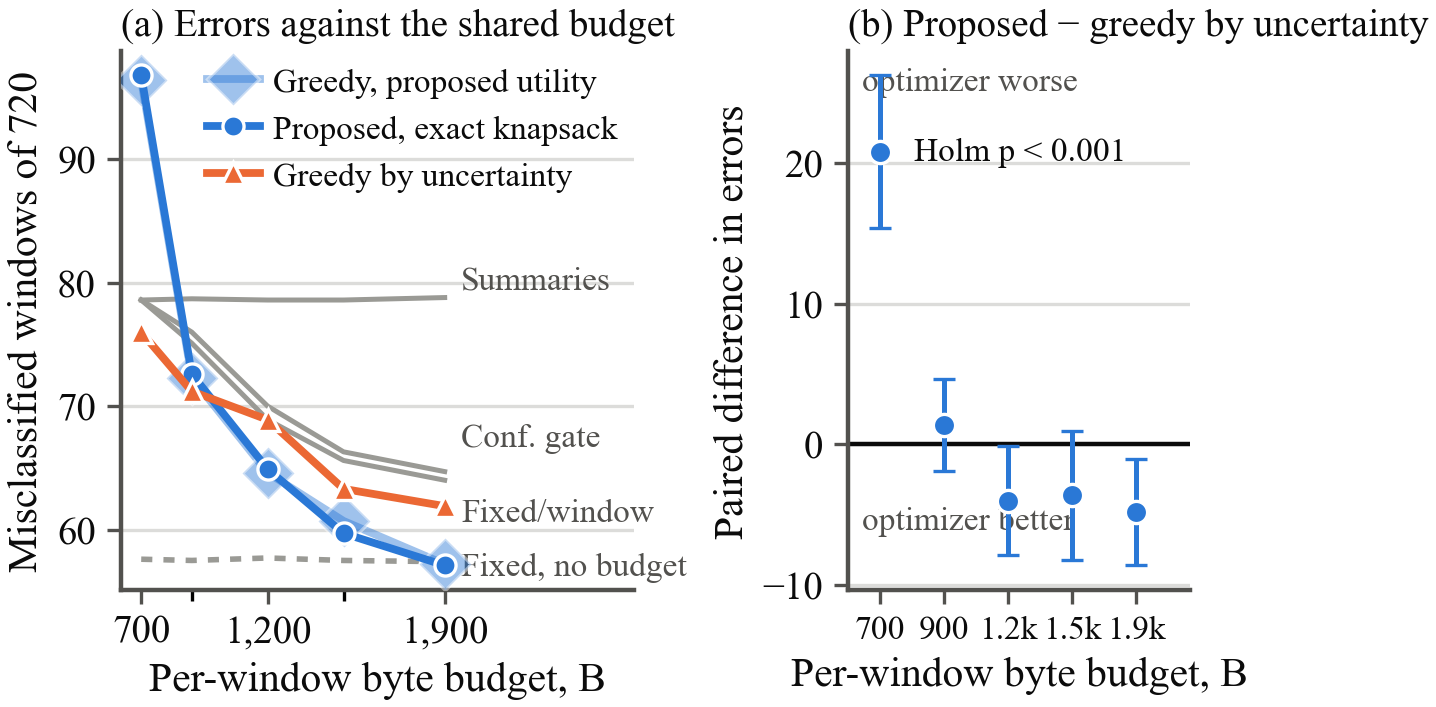
\includegraphics[width=\columnwidth]{fig_contested.png}
\caption{Contested shared budget. (a) Errors against the per-window budget; marginal intervals are omitted because between-seed variation dominates them. The pale diamonds are the greedy heuristic on the proposed utility, which tracks the exact knapsack closely enough to be read as a halo around it. Random-within-budget is omitted because it runs from 140.4 to 109.2 errors; it is in \mtab{tab:contested}{the package}. (b) The paired difference the analysis tests, with 95\% intervals over ten seeds. Only the tight-budget failure survives Holm adjustment.}
\label{fig:contested}
\end{figure}


The tight-budget failure has a clean mechanism. At 700 bytes the optimizer sent nothing for the image in 27\% of windows and nothing for the text in 30\% and held at least one modality in 47\%, in order to buy raw sensor records elsewhere in the slot. It did so because the value function prices a held modality at zero rather than at the cost of losing it. Exact optimization does not repair a misspecified objective; it exploits it more efficiently than a greedy rule can.

A variant designed after these results adds a summary floor: every eligible item is sent at least as a summary and the knapsack chooses only upgrades. We froze a second protocol and tested it on ten new seeds. The floor removed the tight-budget failure. Its advantage over greedy-by-uncertainty replicated in direction at the three largest budgets ($-3.0$, $-3.1$ and $-3.4$ errors) but did not survive adjustment (Holm $p$ 0.087 to 0.353) and was absent at the two tightest budgets ($+0.2$ and $-0.9$). The exact solver again matched a greedy solver with the same floor to within one error. The proposed value function may carry a benefit of roughly 0.4\% of windows at moderate budgets; this benchmark does not establish it and the exact solver contributes nothing measurable.

\ifsubmission
\section{Exploratory Analyses}
\label{sec:exploratory}
These were designed after the confirmatory results and are robustness analyses rather than hypothesis tests, each inheriting the perturbation stream of the condition it modifies: at zero loss, with no trace and with one controller, every method reproduces to every printed digit the run it modifies. The package tabulates all four in full.

\label{sec:forgery}%
\emph{Adversarial metadata.} The admissibility rule~(\ref{eq:adm}) reads metadata and nothing else, so an adversary
who can attach plausible values defeats it by construction. Varying the forged fraction of
misaligned reports collapses the filter almost linearly: worth 7.0 errors against the unfiltered rule's 20.2 with
no forgery, worth nothing at full forgery, 20.2 against 20.2. The admitted fraction tracks
the forged fraction (24.1\%, 48.4\%, 72.4\% against 25\%, 50\%, 75\%); no aligned item is
ever rejected and the optimizer contributes nothing to robustness, tracking the filtered fixed rule within
0.4 to 3.0 errors. There is no safe operating point, so admissibility is a filter against accident rather than a security control; an adversary in the threat model forces signed or attested sources, whose cost belongs in the byte budget. Crossing forgery with a compromised text source pointing 35\% of reports at a wrong class leaves the filtered rule at 19.8 errors, no worse than forgery alone, so forgery alone suffices.

\label{sec:link}%
\emph{Packet loss and a measured link.} Splitting payloads into 1,500-byte packets lost
independently with probability $p$ and retransmitted at a 200~ms timeout leaves accuracy
unmoved, because nothing here ties latency back to the decision, while tail latency is not
unmoved: at 10\% loss the fixed rule goes from 0.09~s to 0.14~s, a factor of 1.5, against
0.57~s to 4.70~s for the policy, a factor of 8.3, widening the gap between them from
6$\times$ to 34$\times$. Replaying measured LTE traces distributed with Mahimahi~\cite{mahimahi} against a constant link of equal mean capacity isolates variability from speed: it inflates tail latency by up to 8.7$\times$. On the Verizon driving trace, whose fifth-percentile throughput falls to 0.25~Mbps, the policy's tail rises from 0.25~s to 2.17~s against 0.24~s to 1.49~s for the fixed rule, so the penalty tracks the depth of the fades rather than the average rate. The tail-latency ranking survives the replay on all three traces; the idea that the optimizer's extra bytes are cheap does not.

\emph{Emulator check.} Every payload of the byte model was then sent over TCP through Mahimahi link shells~\cite{mahimahi} on the three constant links, under the five loss rates and on the three LTE traces beside mean-matched constants, the emulated round trip equal to the scenario's base latency: 2,890 transfers, none failed. The byte term of (\ref{eq:latency}) holds (the 420~kB raw record took 14.05~s on the 256~kbps link against 13.35~s modelled) and the loss stall stays within 13\% up to 5\% loss, 27\% short at 10\%. The additive constant is one round trip short: payloads under 2~kB ran 0.20 to 0.24~s above the model at a 180~ms round trip, 0.08~s at 100~ms and 0.01~s at 40~ms, the connection setup the model omits. On the faster links slow start sets the raw record's time (1.31~s against 0.40~s modelled at 19~Mbps) and the loss term misses both ways on the 10~Mbps link (1.47$\times$ the model at 2\% loss, 0.82$\times$ at 10\%). The Verizon driving trace raised the measured tail 2.0$\times$ over its mean-matched constant, the short trace 1.5$\times$ and the T-Mobile trace 1.0$\times$, the modelled ordering. The byte term the budgeting rests on is confirmed; the fixed overhead and the loss term are not, so latencies small against a round trip are lower bounds.

\label{sec:coord}%
\emph{Coordination.} Dealing a slot's windows round-robin to $C$ independent controllers, each allocating its own windows against a proportional share of an unchanged budget, leaves the two per-window controls unaffected as it must. The coordinated methods separate sharply: removing coordination costs the exact knapsack $+20.0$ errors
$[14.2, 25.8]$ at $B=900$ against $+3.9$ $[0.8, 7.0]$ for the greedy uncertainty ranking, over ten seeds.
The penalty peaks at $B=900$ rather than $B=700$ ($+10.2$), because at 700 bytes the centralised optimizer already fails badly enough that little is left to take away. At $C=6$ the policy makes 92.6 errors against the greedy rule's 75.1, so a rough tie under centralisation becomes a clear loss once the assumption is dropped. The exact optimizer is not merely no better than a greedy ranking; it depends more on an architectural assumption that field deployments are least likely to satisfy.

\label{sec:compute}%
\emph{Compute cost.} Timed as best-of-five wall clock on one workstation with peak allocation recorded and no energy figure inferred, the fixed rule decides a slot in 0.0012~ms against 7.44~ms for the exact knapsack, about 6,190 times longer at 18 times the peak memory. Solve time grows faster than linearly up to four windows sharing a slot and close to linearly beyond six (1: 0.10~ms, 2: 0.42, 3: 0.88, 4: 1.44, 6: 2.37, 8: 3.24, 12: 4.83~ms), approaching the $O(K\cdot64\cdot2000)$ bound once the fixed per-call overhead is amortised. The greedy heuristic on the proposed utility is slower than the exact program, 15.5 against 7.44~ms, only because it is a Python loop while the dynamic program is vectorised.

\else
\section{Exploratory Analyses}
\label{sec:exploratory}
The experiments in this section were designed after the confirmatory results and are reported as robustness analyses, not as hypothesis tests. Each inherits the perturbation stream of the condition it modifies, so it is a controlled comparison rather than a differently drawn workload; we verified that at zero loss, with no trace and with one controller, every method's errors, bytes and latencies equal the earlier values to every printed digit.

\subsection{Adversarial Metadata: The Filter Is Exactly as Strong as Forgery Is Hard}
\label{sec:forgery}
The admissibility rule reads metadata and nothing else, so an adversary who can attach plausible location, time and hazard values to a report defeats it by construction. We hold the misaligned-evidence condition fixed and vary the fraction of misaligned reports whose metadata is set to the target incident's own values. \mtab{tab:forgery}{The full grid, in the package,} shows an almost linear collapse. With no forgery the filter is worth 7.0 errors against 20.2 for the unfiltered rule. With complete forgery it is worth nothing: 20.2 against 20.2. The admitted fraction tracks the forged fraction almost exactly (24.1\%, 48.4\% and 72.4\% against 25\%, 50\% and 75\%), so the rule admits the forged items and nothing else while rejecting no aligned item at any point. The optimizer contributes nothing to robustness: the proposed method tracks the filtered fixed rule within 0.4 to 3.0 errors across the range.

\masteronly{%
\begin{table}[t]
\caption{Errors out of 720 as the share of misaligned reports carrying forged metadata rises, with an uncompromised text source (left) and a compromised source corrupting 35\% of reports (right). Means of five seeds. The 25\% column with an uncompromised source is the reference condition of Section~\ref{sec:adm} and reproduces the five-seed misaligned column it was run against.}
\label{tab:forgery}
\centering\scriptsize
\setlength{\tabcolsep}{2.5pt}
\begin{tabular}{@{}lrrrrrrrrr@{}}
\toprule
 & \multicolumn{5}{c}{Uncompromised source} & \multicolumn{4}{c}{Compromised source} \\
\cmidrule(lr){2-6}\cmidrule(lr){7-10}
Method & 0\% & 25\% & 50\% & 75\% & 100\% & 0\% & 25\% & 50\% & 100\% \\
\midrule
Fixed rule (no filter) & 20.2 & 20.2 & 20.2 & 20.2 & 20.2 & 19.8 & 19.8 & 19.8 & 19.8 \\
Fixed rule + adm.\ & 7.0 & 9.4 & 11.4 & 15.0 & 20.2 & 10.6 & 14.0 & 16.0 & 19.8 \\
Proposed & 6.4 & 8.8 & 10.2 & 12.8 & 17.2 & 10.2 & 12.8 & 14.8 & 18.4 \\
\bottomrule
\end{tabular}
\end{table}}%


Two consequences follow. There is no safe operating point, so a deployment cannot argue that a low expected forgery rate makes the rule sufficient. And metadata admissibility is a cheap filter against accident (misrouted reports, stale caches, misconfigured clients), not a security control; where an adversary is in the threat model it must be backed by signed observations or attested sources, whose cost belongs in the byte budget. We have not evaluated such a scheme and the sweep models metadata substitution only. Crossing the forgery rate with a compromised text source that points 35\% of reports toward a wrong class (the compromised-source half of that grid) shows that forgery alone is sufficient: with both capabilities the filtered rule reaches 19.8 errors, no worse than forgery alone.

\subsection{Packet Loss and a Measured Link}
\label{sec:link}
The results so far treat the link as a constant-rate pipe. Two experiments relax that assumption. The first splits each payload into 1,500-byte packets, each lost independently with probability $p$ and retransmitted, so the bytes placed on the wire grow by $1/(1-p)$ and each lost packet costs one 200~ms retransmission timeout. The expected number of lost packets grows with the payload, so the time penalty is super-linear in bytes. Accuracy is unmoved, because nothing in this condition ties latency back to the decision; tail latency is not unmoved (\mtab{tab:loss}{full grid in the package}). The fixed rule goes from 0.09~s to 0.14~s at 10\% loss, a factor of 1.5; the proposed policy goes from 0.57~s to 4.70~s, a factor of 8.3. The gap between them widens from 6$\times$ to 34$\times$. The optimizer's surplus bytes were close to free under an idealised link; under a lossy one they are the dominant term.

\masteronly{%
\begin{table}[t]
\caption{95th-percentile modelled latency in seconds against packet loss, at the normal per-window budget. *Ignores the budget.}
\label{tab:loss}
\centering\footnotesize
\begin{tabular}{@{}lrrrrr@{}}
\toprule
Method & 0\% & 1\% & 2\% & 5\% & 10\% \\
\midrule
Fixed rule & 0.09 & 0.10 & 0.10 & 0.12 & 0.14 \\
Confidence gate & 0.33 & 0.39 & 0.40 & 0.41 & 0.44 \\
Fixed compression & 0.10 & 0.11 & 0.12 & 0.14 & 0.17 \\
Proposed & 0.57 & 0.83 & 1.23 & 2.47 & 4.70 \\
Transmit all* & 2.24 & 2.89 & 3.64 & 6.12 & 10.72 \\
\bottomrule
\end{tabular}
\end{table}}%


The second experiment replays measured cellular capacity traces in place of the constant rate~\cite{mahimahi}. Each trace records the milliseconds at which one MTU packet could be delivered on a real LTE uplink; we replay them unmodified, varying only the starting offset by slot and compare against a constant link at the same mean capacity, which isolates variability from speed (\mtab{tab:trace}{full grid in the package}). Holding mean capacity fixed, real variability inflates tail latency by up to 8.7$\times$. On the Verizon driving trace, whose fifth-percentile throughput falls to 0.25~Mbps, the proposed policy's tail rises from 0.25~s to 2.17~s and the fixed rule's from 0.24~s to 1.49~s; the steadier traces inflate far less, so the penalty tracks the depth of the fades, not the average rate. Ranking the five methods by tail latency gives the same order under the replayed trace as under its mean-matched constant for all three traces, so the ordering survives the more realistic link; what does not survive is the idea that the optimizer's extra bytes are cheap.

\emph{Emulator check.} The link model was then placed under a real transport. Every payload of the byte model (three summaries, three feature vectors and one raw record per modality at the midpoint of its range) was sent over a TCP connection through Mahimahi link shells~\cite{mahimahi}: the three constant links, the two of them under the five loss rates and the three LTE traces each beside a constant link of the same mean capacity, with the emulated round trip equal to the scenario's base latency; 2,890 transfers in 17 cells, none failed. The byte-proportional term of (\ref{eq:latency}) holds: the 420~kB raw record took 14.05~s on the 256~kbps link against 13.35~s modelled and the loss stall tracked the measurement to within 13\% up to 5\% loss, falling 27\% short at 10\% (26.8 against 21.0~s). The additive constant is one round trip short: payloads under 2~kB measured 0.20 to 0.24~s above the model at a 180~ms round trip, 0.08~s at 100~ms and 0.01~s at 40~ms, which is the connection setup the model omits. On the faster links slow start rather than serialization sets the raw record's time (1.31~s against 0.40~s modelled at 19~Mbps and 180~ms) and the loss term misses in both directions on the 10~Mbps link, the measurement being 1.47$\times$ the model at 2\% loss and 0.82$\times$ at 10\%. Variability acted as the replay predicts: the Verizon driving trace raised the raw record's measured tail 2.0$\times$ over its mean-matched constant, the short trace 1.5$\times$ and the T-Mobile trace 1.0$\times$, the ordering of the modelled column. The byte term on which the budgeting decisions rest is confirmed; the fixed overhead and the loss term are not, so every latency in this paper that is small against a round trip is a lower bound.

\masteronly{%
\begin{table*}[t]
\caption{95th-percentile modelled latency in seconds under a replayed measured LTE trace against a constant link of the same mean capacity. *Ignores the budget.}
\label{tab:trace}
\centering\scriptsize
\setlength{\tabcolsep}{4pt}
\begin{tabular}{@{}lrrrrrrrrr@{}}
\toprule
 & \multicolumn{3}{c}{Verizon short} & \multicolumn{3}{c}{Verizon driving} & \multicolumn{3}{c}{T-Mobile driving} \\
\cmidrule(lr){2-4}\cmidrule(lr){5-7}\cmidrule(lr){8-10}
Method & Const. & Replay & $\times$ & Const. & Replay & $\times$ & Const. & Replay & $\times$ \\
\midrule
Fixed rule & 0.24 & 0.37 & 1.5 & 0.24 & 1.49 & 6.2 & 0.23 & 0.25 & 1.1 \\
Confidence gate & 0.23 & 0.32 & 1.3 & 0.23 & 0.94 & 4.0 & 0.23 & 0.24 & 1.1 \\
Fixed compression & 0.26 & 0.42 & 1.6 & 0.25 & 2.20 & 8.7 & 0.23 & 0.27 & 1.1 \\
Proposed & 0.26 & 0.42 & 1.6 & 0.25 & 2.17 & 8.6 & 0.23 & 0.26 & 1.1 \\
Transmit all* & 3.84 & 7.22 & 1.9 & 3.67 & 20.42 & 5.6 & 1.34 & 3.74 & 2.8 \\
\bottomrule
\end{tabular}
\end{table*}}%


\subsection{Coordination Is Worth More to the Optimizer Than to the Simple Rule}
\label{sec:coord}
Every result so far grants the shared-budget formulation its most favourable assumption: one controller owns all six windows in a slot. An incident area is more plausibly served by several edge nodes that cannot coordinate per slot over the degraded link they are conserving. We deal the slot's windows round-robin to $C$ independent controllers, each allocating only its own windows against a share of the byte budget proportional to the windows it owns. The total budget is unchanged and all controllers still share the physical link. The contested-budget condition is used because it is the only regime in which the shared budget binds; $C=1$ reproduces Table~\ref{tab:contested} exactly.

\masteronly{%
\begin{table}[t]
\caption{Errors out of 720 at $B=900$ bytes as coordination is removed. $C$ is the number of independent controllers sharing one slot. Ten seeds.}
\label{tab:coord}
\centering\footnotesize
\begin{tabular}{@{}lrrrr@{}}
\toprule
Method & $C=1$ & $C=2$ & $C=3$ & $C=6$ \\
\midrule
Summaries only & 78.7 & 78.7 & 78.7 & 78.7 \\
Fixed rule, per window & 75.1 & 75.1 & 75.1 & 75.1 \\
Greedy by uncertainty & 71.2 & 71.4 & 72.0 & 75.1 \\
Proposed (exact knapsack) & 72.6 & 78.3 & 81.5 & 92.6 \\
\bottomrule
\end{tabular}
\end{table}}%


The two per-window methods are controls: they allocate nothing across windows, so $C$ cannot affect them and it does not (\mtab{tab:coord}{full grid in the package}). The two coordinated methods separate sharply. Removing coordination costs the exact knapsack $+20.0$ errors $[14.2, 25.8]$ at $B=900$ and the greedy uncertainty ranking only $+3.9$ $[0.8, 7.0]$. The penalty peaks at $B=900$ rather than at $B=700$ ($+10.2$), because at 700 bytes the centralised optimizer already fails badly enough that little is left to take away. At $C=6$ the proposed method makes 92.6 errors against the greedy rule's 75.1, so a rough tie under centralisation becomes a clear loss once the assumption is dropped. The exact optimizer is not merely no better than a greedy ranking; it is more dependent on an architectural assumption that field deployments are least likely to satisfy and this benchmark charges nothing for the per-slot consensus it would need.

\subsection{What the Policy Costs to Compute}
\label{sec:compute}
We timed the allocation step on the contested-budget views as best-of-five wall clock on one workstation and recorded peak allocation (\mtab{tab:compute}{full table in the package}); no energy figure is inferred. The fixed rule decides a slot in 0.0012~ms; the exact knapsack takes 7.44~ms, about 6,190 times longer and holds 18 times the peak memory. Solve time grows faster than linearly up to four windows sharing a slot and close to linearly beyond six (1: 0.10~ms, 2: 0.42, 3: 0.88, 4: 1.44, 6: 2.37, 8: 3.24, 12: 4.83~ms), approaching the $O(K\cdot64\cdot2000)$ bound once the fixed per-call overhead is amortised. The greedy heuristic on the proposed utility is slower than the exact program (15.5 against 7.44~ms) only because it is a Python loop while the dynamic program is vectorised.

\masteronly{%
\begin{table}[t]
\caption{Measured decision cost at $B=1{,}200$ bytes, per slot and per window. Each seed is timed five times and the fastest run kept; the table reports the mean of five seeds.}
\label{tab:compute}
\centering\scriptsize\setlength{\tabcolsep}{3pt}
\begin{tabular}{@{}p{2.45cm}rrr@{}}
\toprule
Method & Slot (ms) & Window (ms) & Peak (KiB) \\
\midrule
Fixed rule & 0.0012 & 0.0002 & 76 \\
Fixed rule, per window & 0.2070 & 0.0345 & 76 \\
Greedy by uncertainty & 0.4949 & 0.0825 & 180 \\
Greedy, proposed utility & 15.4829 & 2.5805 & 1,329 \\
Proposed (exact knapsack) & 7.4428 & 1.2405 & 1,329 \\
\bottomrule
\end{tabular}
\end{table}}%


\fi
\section{A Reduced Comparison on Real Disaster Data}
\label{sec:real}
Every result above rests on a generated workload; the only measured inputs so far are the capacity traces. This section replaces the synthetic workload with one built from CrisisMMD~\cite{crisismmd}: 3,526 labelled report--image pairs from seven disasters in 2017, with real text, photographs, hazard types, arrival times recovered from the message identifiers, class imbalance and payload sizes. The policies are unchanged and the split is by event. The experiment was designed after the synthetic results, was not pre-registered and is exploratory.

\subsection{Representations and Their Diagnostic}
\label{sec:repr}
Both modalities are represented by CLIP embeddings~\cite{clip}, reduced by principal components fitted on training events only: eight components for text and ten for images, matching the dimensions the policy expects. Measured on the 968 held-out records before any budgeting decision, the image representation reaches 0.566 accuracy against a majority baseline of 0.490, while the text representation returns 0.490, the majority baseline to four decimal places: the text classifier predicts the majority class for every held-out record. A TF--IDF control in the same diagnostic reached the baseline in one of its six cells and fell below it in the other five. These are raw per-record accuracies, not the per-window error counts decided under a budget.

The first submission could not say whether that majority-class outcome was a property of the task, of the eight-component reduction or of class imbalance. A factor diagnostic now separates them. Twenty-five cells were scored on the rotation-0 split, each over five fitting seeds, drawn from five text representations (the eight shipped components, thirty-two components, the full 512-dimension CLIP embedding, a TF--IDF control and the deployed leading-four truncation), three class handlings~\cite{imbalance} (none, balanced class weights, balanced resampling of the training rows) and three classifiers (the package edge model, logistic regression as a floor and the deployed truncation). The decision rule was fixed before the run: the pathway counts as informative under some tested representation only if the best cell clears the majority baseline by more than 0.02 accuracy and exceeds the majority classifier's macro-F1 in at least five of the seven rotations.

The rule returns false on the per-rotation conjunction the protocol records as primary, passing in none of the seven rotations. The best cell, the full CLIP embedding with balanced resampling, raises macro-F1 from the majority classifier's 0.219 to 0.452 on rotation 0 and its macro-F1 gain is positive in all seven rotations, yet its accuracy sits at 0.481 against a majority baseline of 0.490 and is below that baseline in every rotation. Three cells do clear the accuracy bar on rotation 0, by 0.028 to 0.046, all of them without class handling; none survives the rotations, passing in two, two and one of seven. So a better representation does not unlock the pathway. Class handling recovers macro-F1 rather than accuracy: the pathway carries class-discriminative information that an accuracy comparison on imbalanced classes hides, yet still predicts this label too poorly to clear a bar set in advance. The claim this supports is therefore the original one with a sharper reason: on this corpus the text pathway contributes no predictive signal that survives the test fixed in advance, the cause is class imbalance rather than the dimensionality of the reduction and nothing in the value function detects either.

\subsection{What Carries Over}
The comparison is reduced and the data forces the reductions. CrisisMMD has no sensor
stream, so the workload has two modalities and the per-window action space shrinks from 64
combinations to 16, with a fixed-seed placeholder keeping the shared code path running and
the runner asserting the sensor modality is never available. The annotations carry no
geolocation, so the spatial term of~(\ref{eq:adm}) reduces to event identity. No severity
field is independent of the damage label, so severity is held constant and its term is
inert. Imagery is never missing, so the incomplete-modality machinery is not exercised.
Three conditions carry over, not nine. Three methods are absent from Table~\ref{tab:real}, including the fixed
rule with admissibility, so the misaligned condition here cannot isolate the filter as
Section~\ref{sec:adm} does. CrisisMMD carries no delayed imagery, so the derived constant
wait threshold, the clearest positive result of Section~\ref{sec:results}, was untested on
real data in the first submission. It is now tested on a constructed delay drawn per window
from the same log-normal family as the synthetic condition, the seed and the draw recorded
in a protocol frozen before the run, with the protocol's digest in the run manifest. The delay is
therefore declared rather than observed, the honest description of what the corpus allows,
while every other quantity stays real; Section~\ref{sec:realthreshold} reports the outcome.
Five seeds vary model fitting only; the 968 test windows (795 from Hurricane Irma, 173 from the Iraq--Iran earthquake) are identical across them, so intervals bound fitting jitter rather than sampling error and several are zero-width because the method is deterministic given the data. Every published number from here on averages the same five seeds and the reruns below reproduce Table~\ref{tab:real} exactly before any new column is read.

\begin{table}[t]
\caption{All three real-data conditions. Errors out of 968; the majority-class baseline is 494. Bytes and tail latency are for low bandwidth. *Ignores the budget.}
\label{tab:real}
\centering\scriptsize
\setlength{\tabcolsep}{2pt}
\begin{tabular}{@{}p{2.25cm}rrrrr@{}}
\toprule
Method & Normal & Low bw. & Misaligned & Bytes & p95 s \\
\midrule
Image only & 420.0 & 420.0 & 420.0 & 224 & 0.27 \\
Transmit all* & 435.8 & 435.6 & 447.4 & 129,728 & 30.71 \\
Fixed rule & 464.2 & 465.4 & 473.4 & 342 & 0.29 \\
Confidence gate & 437.0 & 465.8 & 474.4 & 1,390 & 0.56 \\
Random within budget & 462.0 & 465.8 & 474.6 & 1,212 & 0.52 \\
Greedy by uncertainty & 466.8 & 466.8 & 476.0 & 2,166 & 0.63 \\
Greedy, proposed utility & 447.0 & 466.8 & 462.2 & 1,896 & 0.63 \\
Proposed (exact knapsack) & 447.0 & 466.8 & 462.2 & 1,896 & 0.63 \\
Fixed compression & 483.0 & 483.0 & 486.0 & 3,072 & 0.80 \\
Text only & 494.0 & 494.0 & 494.0 & 196 & 0.26 \\
\bottomrule
\end{tabular}
\end{table}

\subsection{Results}
\label{sec:realresults}
Against the fixed rule the ranking does not carry over (Table~\ref{tab:real}). The optimizer wins under normal connectivity by 17.2 errors $[15.8, 18.6]$ and under misaligned evidence by 11.2 $[7.8, 14.6]$ and loses only under low bandwidth, by 1.4 $[0.7, 2.1]$, which is 0.14\% of the test set. Reporting only the low-bandwidth column would have reproduced the synthetic conclusion by selection. One assignment of seven events to three splits produced that pattern and the test set is dominated by one hurricane, so we rotated the event list through seven pre-specified assignments, each keeping the same 3/2/2 shape, so that every event serves in the test set at least once (\mtab{tab:rotation}{the per-rotation differences are tabulated in the package}). The rotations were fixed before running and none was discarded. The direction survives the rotation and the per-condition pattern does not. The optimizer is ahead of the fixed rule in 15 of the 21 comparisons and under normal connectivity in every one of the seven, but the loss under low bandwidth occurs in 2 rotations of 7 and the win under misaligned evidence in 3. What generalises from this corpus is therefore narrower than Table~\ref{tab:real} alone suggests: on real data the optimizer is ahead of the fixed rule more often than not, decisively so when the link is not the constraint and which way any single condition falls depends on which disasters land in the test set.

\masteronly{%
\begin{table}[t]
\caption{Proposed minus fixed rule in errors, by event split. Negative means the optimizer wins. Rotation 0 is the split of Table~\ref{tab:real}. Counts differ because the events differ in size.}
\label{tab:rotation}
\centering\scriptsize\setlength{\tabcolsep}{3pt}
\begin{tabular}{@{}lp{2.05cm}rrrr@{}}
\toprule
Rot. & Test events & $n$ & Normal & Low bw. & Misaligned \\
\midrule
0 & Irma + Iraq--Iran & 968 & $-17.2$ & $+1.4$ & $-11.2$ \\
1 & Harvey + Iraq--Iran & 1,065 & $-3.0$ & $-5.4$ & $+2.8$ \\
2 & Harvey + Maria & 1,754 & $-0.2$ & $+1.0$ & $+1.6$ \\
3 & California + Maria & 1,393 & $-18.8$ & $-12.8$ & $+8.2$ \\
4 & California + Mexico & 709 & $-3.0$ & $-1.0$ & $+18.8$ \\
5 & Mexico + Sri Lanka & 273 & $-7.6$ & $-8.6$ & $-6.4$ \\
6 & Irma + Sri Lanka & 890 & $-57.2$ & $-33.2$ & $-47.6$ \\
\bottomrule
\end{tabular}
\end{table}}%
The comparison that matters most for this paper is between the exact solver and a greedy heuristic on the same utility; on real data the two are identical: the same errors, bytes per window and 95th-percentile latency in all three conditions and at every seed, a paired difference of exactly 0.0. A greedy ranking by local uncertainty, which does not use the utility, makes 466.8 errors under normal connectivity against 447.0, so the utility is doing work even though the solver is not (Fig.~\ref{fig:real}).

\begin{figure}[t]
\centering
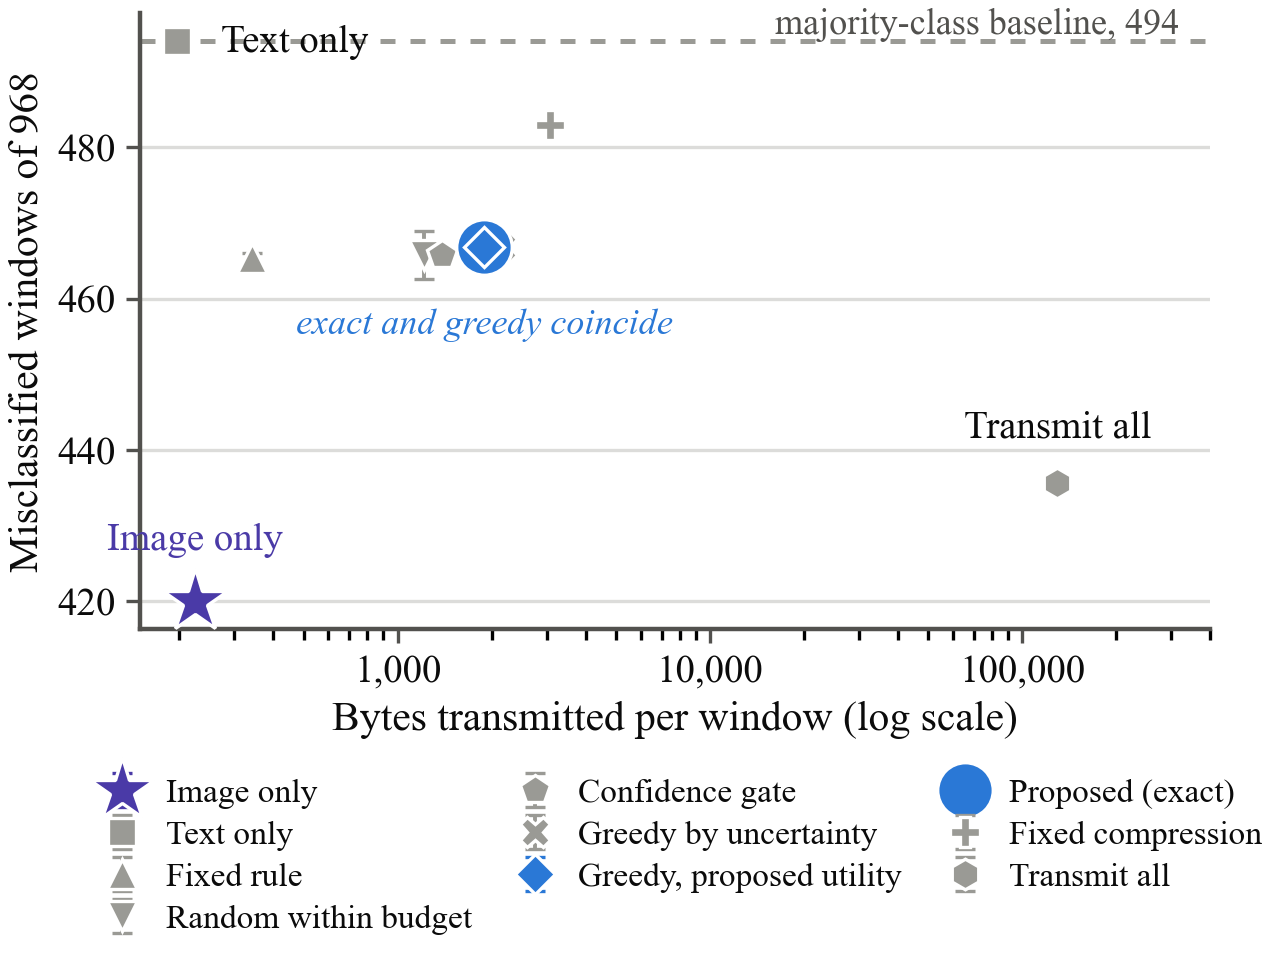
\includegraphics[width=\columnwidth]{fig_real_scatter.png}
\caption{Errors against bytes on real data under low bandwidth. Intervals are fitting jitter across five seeds on one fixed test set and are zero-width for the deterministic methods. The exact knapsack and the greedy heuristic over the same utility occupy the same point.}
\label{fig:real}
\end{figure}


What beats everything on errors is image-only, at 420.0 in every condition, ahead of the optimizer by 46.8 errors $[46.2, 47.4]$ under low bandwidth while sending 224 bytes. Its value cannot vary, because the conditions perturb text and bandwidth while image-only is sensitive to neither, so its constancy is not robustness; the same method makes 71.5 errors against the fixed rule's 5.2 on the synthetic benchmark, so a method near-worst on one workload and best on the other is telling us about the workloads. The reason is in the same table: text-only scores the majority-class count, 494.0, in every condition and everything fusing text pays for it. Severity, reliability, recency, fidelity, uncertainty, quality and disagreement are properties of the source or the signal; none asks whether this modality has ever predicted this label, which a held-out estimate of predictive contribution would. Transmit-all is also ahead on errors, by 31.2 $[30.2, 32.2]$, while sending 129,728 bytes against 1,896 at 30.7~s of tail latency against 0.63~s.

Two assumptions do not survive the move. Conformal coverage, which held between 0.889 and 0.899 across the synthetic conditions, falls to 0.816 under normal connectivity and 0.745 under low bandwidth against a nominal 0.90. Calibration and test windows come from different disasters, so the exchangeability that Proposition~\ref{prop:coverage} assumes fails within a condition; per-condition recalibration cannot repair that and the 7.2-point spread across the three conditions shows a condition-dependent component this explanation does not account for. The byte model of Section~\ref{sec:workload} is contradicted by measurement: real images run from 1,763 to 1,719,070 bytes with a median of 103,142.5 against an assumed 220,000 to 620,000, so the assumed range is both too narrow and centred too high and every report is smaller than the smallest summary the method defines, 39 to 181 bytes against an assumed 350 to 1,800. Sending a report verbatim is cheaper than summarising it, so the summarise-or-send decision is vacuous for that modality on this corpus. Byte sizes are measurable before a budget is designed around them.

\subsection{The Constant Threshold on Real Data}
\label{sec:realthreshold}
The derived constant threshold is the clearest positive result of the synthetic benchmark, so it is the one worth testing hardest. CrisisMMD carries no delayed imagery, so the arrival delay is constructed from the same log-normal family as the synthetic condition, drawn once from a protocol frozen before the run, with the protocol's digest in the run manifest; every other quantity stays as the corpus supplies it. $T^\ast$ is computed on calibration events only, as (\ref{eq:tstar}) defines it, landing between 164.0 and 186.8~s across the rotations.

\masteronly{%
\begin{table}[t]
\caption{The constant threshold on real data, by event rotation. $T^\ast$ is derived on the calibration events of each rotation; 95th-percentile latency in seconds and errors out of the rotation's test windows (Table~\ref{tab:rotation} gives $n$) for the threshold rule, the always-wait rules (fixed rule and wait-if-uncertain coincide) and the proposed policy, means of five seeds. Source: results/real\_delay\_rev2.csv.}
\label{tab:realthr}
\centering\scriptsize\setlength{\tabcolsep}{3.5pt}
\begin{tabular}{@{}lrrrrrr@{}}
\toprule
& & \multicolumn{2}{c}{p95 latency, s} & \multicolumn{3}{c}{Errors} \\
\cmidrule(lr){3-4}\cmidrule(lr){5-7}
Rot. & $T^\ast$, s & Threshold & Always wait & Threshold & Always wait & Policy \\
\midrule
0 & 178.4 & 25.4 & 1,833.9 & 486.0 & 451.0 & 486.0 \\
1 & 180.0 & 25.8 & 1,914.8 & 355.0 & 371.0 & 358.2 \\
2 & 180.2 & 25.8 & 1,800.5 & 689.0 & 691.8 & 690.0 \\
3 & 186.8 & 25.1 & 1,739.2 & 445.4 & 430.0 & 442.6 \\
4 & 184.2 & 25.1 & 1,830.7 & 95.0 & 109.0 & 98.0 \\
5 & 181.5 & 26.8 & 1,791.1 & 71.0 & 80.0 & 67.0 \\
6 & 164.0 & 25.7 & 1,739.4 & 503.0 & 466.8 & 494.0 \\
\bottomrule
\end{tabular}
\end{table}}%

The latency half carries over and the accuracy half does not. On rotation 0 the threshold rule holds 95th-percentile latency at 25.4~s where the always-wait rules reach 1,833.9~s, a factor of 72; in all seven rotations it holds 25.1 to 26.8~s against 1,739.2 to 1,914.8~s\masteronly{ (Table~\ref{tab:realthr})}. Against the always-wait rules it costs 35.0 errors on rotation 0 (486.0 against 451.0 out of 968) and ranges from 16.0 fewer to 36.2 more across the seven. Against the proposed policy, the comparator the pre-specified rule names, its error count lies inside the policy's paired interval in one rotation where five were required, so the rule returns \emph{does not carry over}; those intervals are narrow because the method is deterministic given the data; the threshold rule has fewer errors than the policy in three rotations, the same in one and more in three. Acting early improved accuracy on the synthetic benchmark only because that benchmark decays the weight of evidence while a decision waits (Section~\ref{sec:delay}). The real corpus has no such decay, so waiting costs nothing in evidence quality and the latency saved is bought with accuracy rather than alongside it.

The fixed rule and wait-if-uncertain coincide here at every seed and rotation because wait-if-uncertain's branch (text and sensor confidence below 0.90, which on this two-modality corpus is text confidence alone) fires on every window, so the baseline meant to ignore the forecast collapses into the one that always waits and is not a comparison.

\subsection{Class Imbalance in the Budgeting Pipeline}
\label{sec:realimbalance}
Section~\ref{sec:repr} attributes the text pathway's behaviour to class imbalance, so the question is what the budgeting comparison does when the imbalance is handled everywhere rather than only diagnosed. Balanced resampling~\cite{imbalance}, the handling the diagnostic selected, was applied to every per-modality edge and cloud model before the comparison was rerun. The unhandled column reproduces all ten methods of Table~\ref{tab:real} exactly, which is the precondition for reading the handled column.\masteronly{ Per-method values are in Table~\ref{tab:handled}.}

\masteronly{%
\begin{table}[t]
\caption{Class handling in the budgeting pipeline. Errors out of 968 under normal connectivity on rotation 0, means of five seeds, for the deployed pipeline (current) and with balanced resampling applied to every per-modality model (handled). Source: results/crisismmd\_budgeting\_rev2.csv.}
\label{tab:handled}
\centering\scriptsize\setlength{\tabcolsep}{5pt}
\begin{tabular}{@{}lrrr@{}}
\toprule
Method & Current & Handled & Change \\
\midrule
Image only & 420.0 & 466.6 & $+46.6$ \\
Text only & 494.0 & 576.4 & $+82.4$ \\
Transmit all & 435.8 & 377.8 & $-58.0$ \\
Confidence gate & 437.0 & 377.4 & $-59.6$ \\
Fixed compression & 483.0 & 502.2 & $+19.2$ \\
Fixed rule & 464.2 & 498.2 & $+34.0$ \\
Random within budget & 462.0 & 484.8 & $+22.8$ \\
Greedy by uncertainty & 466.8 & 501.0 & $+34.2$ \\
Greedy, proposed utility & 447.0 & 385.6 & $-61.4$ \\
Proposed (exact knapsack) & 447.0 & 385.6 & $-61.4$ \\
\bottomrule
\end{tabular}
\end{table}}%

The direction of the headline claim survives and its magnitude does not. The optimizer
stays ahead of the fixed rule in 14 of the 21 comparisons against 15 without handling, together with all seven rotations under normal connectivity in both columns. The sizes move far more
than that count suggests: under normal connectivity on rotation 0 the gap widens from
$-17.2$ errors to $-112.6$. The optimizer
improves from 447.0 to 385.6 errors and transmit-all
from 435.8 to 377.8, while every single-modality rule gets worse, text-only from 494.0 to
576.4 and image-only from 420.0 to 466.6. Handling the imbalance makes the fused
prediction better and the single-modality prediction worse, which is consistent with
resampling trading majority-class accuracy for minority-class recall. The comparison is
thus sensitive to class handling in size while not in sign. The single-modality rule
that beats everything in Table~\ref{tab:real} does so partly because the imbalance was
left in place.

\subsection{A Label the Paper Did Not Choose}
\label{sec:reallabel}
Every real-data number above scores the damage label annotated from the photograph, which is this paper's own choice, so the sharpest available test is to replace it with one the dataset's annotators defined. CrisisMMD labels every record with a humanitarian category independently of the damage field~\cite{crisismmd}. The decision machinery is fixed at three classes, so the task is restricted to the three most frequent, keeping 2,763 of 3,526 records in three categories: other relevant information; infrastructure and utility damage; rescue, volunteering or donation effort. \ifsubmission The five categories dropped are: not humanitarian (398 records), injured or dead people (187), affected individuals (150), vehicle damage (21) and missing or found people (7). \else The caption of Table~\ref{tab:extlabel} lists the five discarded categories. \fi On the two tasks that~\cite{ofli2020} publish (informative against not-informative; five humanitarian categories) on their agreed-label splits, this representation with a logistic-regression head chosen on the development split reaches 93.7\% and 88.9\% test accuracy from both modalities and 87.9\% and 83.4\% from text alone, against the published 84.4\% and 78.4\%; the reduced 8- and 10-component form reaches 91.5\% and 87.7\%. The text pathway that is majority-class on the damage label carries signal on the published labels, so the deficiency lies in that label and its imbalance rather than in the encoder.

This is where the comparison fails. On the annotators' label the optimizer is ahead of the
fixed rule in 11 of the 21 comparisons rather than 15, together with 3 of the 7 rotations under
normal connectivity rather than all 7. With the class handling of
Section~\ref{sec:realimbalance} applied as well it is ahead in 8 of 21. The claim in
Section~\ref{sec:realresults} that survives the event rotation, that the optimizer is
ahead under normal connectivity in every one of the seven, does not survive a change of
label on the same records, the same splits and the same conditions. What generalises from
this corpus is therefore narrower again than the rotation analysis alone establishes: the
direction of the real-data result is a property of the label as much as of the method, so a deployment cannot read Table~\ref{tab:real} as evidence that the optimizer will lead on
its own labelling.

\masteronly{%
\begin{table}[t]
\caption{The externally defined label. Proposed minus fixed rule in errors by rotation,
negative means the optimizer wins, on the three most frequent CrisisMMD humanitarian
categories. Current is the deployed pipeline; handled applies the balanced resampling of
Section~\ref{sec:realimbalance}. Discarded categories: not humanitarian (398 records),
injured or dead people (187), affected individuals (150), vehicle damage (21), missing or
found people (7). $n$ is the rotation's test size, smaller than in Table~\ref{tab:rotation} because the three retained categories keep 2,763 of 3,526 records, so magnitudes are not comparable across the two tables.}
\label{tab:extlabel}
\centering\footnotesize
\begin{tabular}{@{}lrrrrrrr@{}}
\toprule
& & \multicolumn{2}{c}{Normal} & \multicolumn{2}{c}{Low bw.} & \multicolumn{2}{c}{Misaligned} \\
\cmidrule(lr){3-4}\cmidrule(lr){5-6}\cmidrule(lr){7-8}
Rot. & $n$ & Curr. & Hand. & Curr. & Hand. & Curr. & Hand. \\
\midrule
0 & 780 & $-8.0$ & $+0.4$ & $-1.8$ & $+1.2$ & $-3.8$ & $+23.2$ \\
1 & 842 & $-10.4$ & $+10.0$ & $-13.2$ & $+17.0$ & $-15.8$ & $+18.2$ \\
2 & 1,362 & $+9.8$ & $-21.0$ & $-27.0$ & $-24.0$ & $-57.8$ & $-14.8$ \\
3 & 1,056 & $+7.4$ & $-7.0$ & $+14.2$ & $+11.2$ & $-4.4$ & $+9.8$ \\
4 & 556 & $+19.6$ & $+100.6$ & $+8.6$ & $+119.8$ & $-3.8$ & $+102.0$ \\
5 & 199 & $0.0$ & $-3.4$ & $+1.0$ & $+1.4$ & $+1.4$ & $+1.2$ \\
6 & 731 & $-3.0$ & $-4.2$ & $+12.0$ & $-22.0$ & $+4.8$ & $-13.6$ \\
\midrule
Ahead & & 3/7 & 4/7 & 3/7 & 2/7 & 5/7 & 2/7 \\
\bottomrule
\end{tabular}
\end{table}}%


\section{What the Evidence Supports}
One conclusion holds across both workloads: the value of this formulation is not in its solver. On real data a greedy heuristic over the proposed utility returned the exact program's allocation at every seed, a paired difference of exactly zero. At twenty seeds the optimizer is indistinguishable from the fixed rule wherever the budget alone binds and leads it where waiting, admissibility or degraded evidence is in play, which corrects the five-seed reading this paper previously gave without rescuing the solver: the gain comes from the threshold rule with the admissibility filter, both supplied by the formulation with no solver at all. It earns its place by naming the quantities that matter and supplying the threshold (\ref{eq:threshold}) that turns them into a rule. What does not hold across both workloads is the ranking. On real data the optimizer leads the fixed rule in 15 of 21 comparisons on the label this paper chose, 14 of 21 once class imbalance is handled everywhere and 11 of 21 on the annotators' own label, where its lead under normal connectivity falls from all seven splits to three. Which simple rule wins is therefore a property of the workload, of the class handling and of the labelling, so the rule has to be derived and tested against held-out data from the deployment, labelled the way the deployment labels it. \ifsubmission Seven deployment checks follow from these results and are set out in the package.\else
Seven checks follow, all within the simulation scope of this study. \emph{One}, derive the
candidates, a byte-profile fixed rule, the constant threshold~(\ref{eq:tstar}) and a greedy
ranking with a summary floor where a shared budget binds, then choose among them on
held-out events, keeping the exact optimizer only if it beats all three. \emph{Two}, before
optimizing a value function check what it prices at zero; the tight-budget failure was a
misspecification that exact optimization exploited. \emph{Three}, treat metadata
admissibility as protection against accident rather than adversaries, its value falling
linearly with forging capability. \emph{Four}, recalibrate conformal thresholds per
operating condition and across the event boundary the deployment will cross, sizing the
review queue from reviewer capacity. \emph{Five}, check whether a shared-budget method
still helps when controllers cannot coordinate; the exact knapsack lost far more than a
greedy ranking. \emph{Six}, add a held-out estimate of predictive contribution to the value
function, since no existing term detects a modality carrying no signal for the label. Handle
class imbalance in every per-modality model before reading the comparison: doing so
left the direction of the real-data result intact while moving one rotation's gap from
$-17.2$ to $-112.6$ errors and reversing which methods benefit. \emph{Seven}, score the
comparison on more than one labelling of the same records; the result here held across
seven event splits yet not across a change of label, so an event rotation alone does not
establish that a ranking will transfer.

\fi



\section{Limitations and Threats to Validity}
\label{sec:limits}
The verification data are synthetic and well separated, which explains error rates below 1\% for the stronger methods and makes the conformal sets nearly binary. Byte sizes, delay distributions, forecast errors and the rate at which evidence ages are assumptions on which the conclusions about fixed rules and waiting depend; Section~\ref{sec:delay} shows the accuracy result under delay disappearing when evidence does not age. Section~\ref{sec:real} removes a smaller part of this limitation than ``real data'' suggests: the link, budgets, loss model, slot structure, sensor modality and severity stay synthetic or fixed, six of nine conditions and three of eleven methods do not carry over and the arrival delay used to test the wait threshold on that corpus is constructed rather than observed. The text pathway's majority-class outcome is no longer unresolved: a twenty-five-cell diagnostic attributes it to class imbalance rather than to the dimensionality of the reduction, with no tested representation clearing a bar fixed in advance in more than two of seven splits.

The link model is the sharpest limitation for an edge-systems audience. Loss, retransmission and replayed measured capacity narrow it and the emulator check of Section~\ref{sec:exploratory} puts a real TCP stack under the model; there is still no MAC layer, routing, contention between nodes or radio. There is no hardware testbed and no energy measurement; Section~\ref{sec:compute} reports wall-clock time and peak allocation on one workstation and we decline to infer joules from them. Section~\ref{sec:coord} relaxes the single-controller assumption by static partitioning only. Every statement in this paper about edge deployment is therefore bounded by simulation and emulation on a workstation.

Policy coefficients and thresholds were set by hand; the latency penalty is accompanied by a sweep and the main protocol was not pre-registered. The admissibility test favours the filter by construction. The contested-budget difficulty was chosen by a rule fixed in advance, but the budget grid and the competitor were chosen by the authors and both protocols are timestamped only within the package. The severity estimator is weak, so severity-dependent behaviour is barely exercised. Twenty seeds and four test events per seed still limit statistical resolution: three of the eight paired error comparisons include zero, so we treat those three as inconclusive rather than as equivalence. On the real-data side the seeds vary model fitting only, which is why we rotate the event split; the seven assignments reuse the same events and are not independent. Social-media and sensor sources carry participation and placement bias. Improved disaster outcomes cannot be claimed without measured network traces, more disasters and prospective studies with emergency-management partners.


Two tests could not be completed on the available inputs, so we state the grounds. Reproducing the published CrisisMMD baselines~\cite{crisismmd} on the official split needs published values for the damage task and none exist: the baselines of~\cite{ofli2020} exclude damage severity because it was annotated on images alone. The official damage split was obtained: the same 3,526 records, divided 2,468/529/529 rather than by event. The established tasks cannot run through the budgeting pipeline at their published cardinality because the reference implementation is fixed at three classes and is carried unchanged so its published numbers stay checkable; Section~\ref{sec:reallabel} scores the representation on them instead.

\section{Reproducibility, Oversight and Data Availability}
The package contains source, environment lock, configuration, split identifiers, calibration temperatures, thresholds, seeds, integrity tests, record-level predictions for every method and condition, provenance envelopes, the two frozen contested-budget protocols with SHA-256 digests and scripts that regenerate every table and figure. On one CPU architecture reruns reproduce every output file byte for byte across Python 3.12 to 3.14. Across architectures about 10\% of source observation vectors differ in their last bits (the generator's Beta and Dirichlet draws reach platform libm); no reported quantity, all written at six significant figures or fewer, is affected and the provenance digest is taken over observations rounded to nine decimals. The real-data pipeline depends on a pretrained encoder and on PyTorch, whose versions are not pinned. Re-deriving the records from the source archive with a later stack reproduced the labels, splits, arrival times, byte sizes, quality signals and all eight text components exactly; the ten image components moved by at most 0.13 (under 1\% of their spread) and Table~\ref{tab:real} rerun on those records changed no cell by more than 1.0 error in 968 and no paired difference by more than 1.8 with every sign preserved, bytes and latency unchanged. Byte-for-byte reproduction of the image components is therefore not claimed; the results reported from them are. The package changelog lists design errors corrected during development; results from before those corrections are superseded.

The method is decision support, not an autonomous responder. Reviewers receive the evidence set, the uncertainty, the conflict indicators, the reason codes and the status rule that fired; the interface must distinguish observed evidence from model-derived fields. Governance follows the NIST AI RMF lifecycle~\cite{nistrmf}; deployment requires agency authority, privacy and cybersecurity review, periodic recalibration (Section~\ref{sec:coverage}) and a staffing plan for the queue of Section~\ref{sec:queue}. Raw transmission must be policy-gated.

The package is maintained at \url{https://github.com/bdata-arindam/Edge} at version 2.6.17, the version behind every result reported here, whose \texttt{SHA256SUMS} records a digest for each of its 113 files. {\edef\tmpdoi{\archivedoi}\ifx\tmpdoi\empty\else The archived release is \texttt{\archivedoi}. \fi}The emulator scripts and transfer log are held with the manuscript materials outside the frozen package. The synthetic verification contains no personal data. Section~\ref{sec:real} uses CrisisMMD v2.0, obtained from its authors under their terms and not redistributed; we ship derived features, byte counts and labels, not the posts or images. Operational use of field reports or agency data would require institutional, legal and privacy review.

\section{Conclusion}
We formulated disaster evidence transmission as a shared-budget knapsack across concurrent
incidents in which waiting for late evidence is an explicit decision with a delay threshold
and admissibility is checked before any evidence is valued or fused. On the synthetic
benchmark at twenty seeds the simple rules the formulation generates are indistinguishable
from the optimizer wherever the budget alone binds; a pre-registered test found the
optimizer worse than its competitor at the tightest budget while one of its five
differences survived adjustment in the solver's favour, by one error in 720; the
admissibility filter's protection falls to nothing in proportion to an adversary's ability
to forge metadata; and the conformal guarantee does not transfer across conditions. On real
data the optimizer's lead over the fixed rule falls from 15 of 21 comparisons on the damage
label this paper chose to 14 of 21 once class imbalance is handled and to 11 of 21 on the annotators' own, where under normal connectivity it falls from all seven event splits to three; a single-modality rule beats everything on the chosen label, partly because the imbalance was left in place. The text pathway is diagnosed: its majority-class behaviour is a
class-imbalance effect rather than an artefact of the reduction, no tested representation
clears a bar fixed in advance and the value function detects none of it. The delay
threshold keeps a 67- to 74-fold tail-latency reduction in every split while its accuracy gain does not carry over, because that corpus does not decay evidence while a decision waits.
What survives both workloads is that the formulation earns its place by naming the
quantities that matter and supplying the threshold that turns them into a rule, never by
the solver. Which simple rule to deploy has to be derived against the data a system will
see and scored on the labelling that system will use. An emulated TCP path confirms the latency model's byte term and finds its fixed overhead one round trip short; field value on edge hardware and radios remains to be established.

\masteronly{%
\begin{table}[!t]
\caption{Proposed (P), fixed rule (FR) and transmit all (TA) across every synthetic condition, mean of twenty seeds. Errors out of 720; bytes per window; 95th-percentile modelled latency in seconds. Every row comes from the same twenty-seed run, so this table shares its seed basis with Tables~\ref{tab:lowbw} and~\ref{tab:delay}.}
\label{tab:allcond}
\centering\scriptsize\setlength{\tabcolsep}{1.6pt}
\begin{tabular}{@{}p{1.55cm}rrrrrrr@{}}
\toprule
Condition & Err P & Err FR & Err TA & Bytes P & Bytes FR & p95 P & p95 FR \\
\midrule
Normal & 4.6 & 5.2 & 4.4 & 50,928 & 1,860 & 0.60 & 0.09 \\
Low bandwidth & 4.4 & 5.2 & 4.3 & 3,604 & 1,860 & 0.92 & 0.59 \\
Delayed imagery & 10.2 & 23.4 & 19.2 & 2,393 & 1,860 & 364.85 & 1,864.41 \\
Outage & 4.5 & 5.2 & 4.4 & 3,684 & 1,860 & 13.87 & 13.71 \\
Image missing & 14.1 & 14.1 & 14.1 & 1,636 & 1,636 & 0.19 & 0.19 \\
Text missing & 17.2 & 20.0 & 17.6 & 2,608 & 784 & 0.21 & 0.16 \\
Noisy text & 6.5 & 7.8 & 7.0 & 3,684 & 1,860 & 0.24 & 0.19 \\
Contradictory & 13.8 & 16.3 & 14.1 & 3,684 & 1,860 & 0.24 & 0.19 \\
Misaligned & 13.9 & 35.0 & 30.8 & 3,448 & 1,860 & 0.23 & 0.19 \\
\bottomrule
\end{tabular}
\end{table}}%


\masteronly{%
\begin{table}[!t]
\caption{Component ablations at twenty seeds (component removed from policy and fusion; positive means it helped; severity replaced by its training mean). Seven of the eleven ablations are distinguishable from zero at twenty seeds against three of eleven at five; the four exact zeros are components the condition does not exercise. Rows are ordered by the magnitude of the effect.}
\label{tab:ablation}
\centering\footnotesize
\begin{tabular}{@{}lr@{}}
\toprule
Component (condition) & $\Delta$ errors, ablated minus full [95\% CI] \\
\midrule
Severity (low bandwidth) & $+0.00$ [0.00, 0.00] \\
Severity (normal) & $+0.00$ [0.00, 0.00] \\
Novelty (contradictory) & $+0.00$ [0.00, 0.00] \\
Novelty (noisy text) & $+0.00$ [0.00, 0.00] \\
Reliability (noisy text) & $-0.45$ [$-0.89$, $-0.01$] \\
Recency (delayed) & $-0.50$ [$-0.99$, $-0.01$] \\
Reliability (contradictory) & $+2.75$ [1.71, 3.79] \\
Quality (contradictory) & $+2.80$ [1.52, 4.08] \\
Quality (noisy text) & $+3.45$ [2.35, 4.55] \\
Latency penalty (delayed) & $+9.05$ [5.64, 12.46] \\
Admissibility (misaligned) & $+16.20$ [11.07, 21.33] \\
\bottomrule
\end{tabular}
\end{table}}%


\begin{thebibliography}{00}
% A long unbreakable token such as an arXiv identifier cannot be hyphenated, so a narrow
% column can force loose lines. A little extra stretch avoids that without touching the
% prescribed fonts or margins.
\bibitem{xbd}
R. Gupta et al., ``Creating xBD: A dataset for assessing building damage from satellite imagery,'' in \emph{Proc. IEEE/CVF Conf. Comput. Vis. Pattern Recognit. Workshops (CVPRW)}, 2019, pp. 10--17.
\bibitem{floodnet}
M. Rahnemoonfar, T. Chowdhury, A. Sarkar, D. Varshney, M. Yari, and R. R. Murphy, ``FloodNet: A high resolution aerial imagery dataset for post flood scene understanding,'' \emph{IEEE Access}, vol. 9, pp. 89644--89654, 2021, doi: 10.1109/ACCESS.2021.3090981.
\bibitem{sen1floods}
D. Bonafilia, B. Tellman, T. Anderson, and E. Issenberg, ``Sen1Floods11: A georeferenced dataset to train and test deep learning flood algorithms for Sentinel-1,'' in \emph{Proc. IEEE/CVF Conf. Comput. Vis. Pattern Recognit. Workshops (CVPRW)}, 2020, pp. 835--845, doi: 10.1109/CVPRW50498.2020.00113.
\bibitem{crisismmd}
F. Alam, F. Ofli, and M. Imran, ``CrisisMMD: Multimodal Twitter datasets from natural disasters,'' in \emph{Proc. 12th Int. AAAI Conf. Web Social Media (ICWSM)}, 2018.
\bibitem{ofli2020}
F. Ofli, F. Alam, and M. Imran, ``Analysis of social media data using multimodal deep learning for disaster response,'' in \emph{Proc. 17th Int. Conf. Inf. Syst. Crisis Response Manage. (ISCRAM)}, 2020.
\bibitem{shi2016}
W. Shi, J. Cao, Q. Zhang, Y. Li, and L. Xu, ``Edge computing: Vision and challenges,'' \emph{IEEE Internet Things J.}, vol. 3, no. 5, pp. 637--646, 2016.
\bibitem{satya2017}
M. Satyanarayanan, ``The emergence of edge computing,'' \emph{Computer}, vol. 50, no. 1, pp. 30--39, 2017.
\bibitem{neurosurgeon}
Y. Kang et al., ``Neurosurgeon: Collaborative intelligence between the cloud and mobile edge,'' in \emph{Proc. 22nd ACM Int. Conf. Archit. Support Program. Lang. Oper. Syst. (ASPLOS)}, 2017, pp. 615--629, doi: 10.1145/3037697.3037698.
\bibitem{shi2020}
Y. Shi, K. Yang, T. Jiang, J. Zhang, and K. B. Letaief, ``Communication-efficient edge AI: Algorithms and systems,'' \emph{IEEE Commun. Surveys Tuts.}, vol. 22, no. 4, pp. 2167--2191, 2020.
\bibitem{dat}
Q. Guo, Z. Yang, Y. Hu, C. Zhao, and W. Ji, ``DAT: Dual-aware adaptive transmission for efficient multimodal LLM inference in edge-cloud systems,'' 2026, arXiv:2604.05375.
\bibitem{cst}
H. Chi et al., ``CST: Collaborative selective transmission for communication-efficient multimodal edge inference,'' 2026, arXiv:2608.22115.
\bibitem{avery}
R. Bhattacharjya et al., ``AVERY: Intent-driven adaptive VLM split computing via embodied self-awareness for efficient disaster response systems,'' Nov. 2025, arXiv:2511.18151v1.
\bibitem{chen2023}
Y. Chen, M. Zhao, and L. Bruzzone, ``Incomplete multimodal learning for remote sensing data fusion,'' 2023, arXiv:2304.11381.
\bibitem{guo2017}
C. Guo, G. Pleiss, Y. Sun, and K. Q. Weinberger, ``On calibration of modern neural networks,'' in \emph{Proc. 34th Int. Conf. Mach. Learn. (ICML)}, 2017, pp. 1321--1330.
\bibitem{selectivenet}
Y. Geifman and R. El-Yaniv, ``SelectiveNet: A deep neural network with an integrated reject option,'' in \emph{Proc. 36th Int. Conf. Mach. Learn. (ICML)}, 2019, pp. 2151--2159.
\bibitem{sadinle}
M. Sadinle, J. Lei, and L. Wasserman, ``Least ambiguous set-valued classifiers with bounded error levels,'' \emph{J. Amer. Statist. Assoc.}, vol. 114, no. 525, pp. 223--234, 2019.
\bibitem{romano}
Y. Romano, M. Sesia, and E. Cand\`es, ``Classification with valid and adaptive coverage,'' in \emph{Proc. Adv. Neural Inf. Process. Syst. (NeurIPS)}, vol. 33, 2020, pp. 3581--3591.
\bibitem{ovadia}
Y. Ovadia et al., ``Can you trust your model's uncertainty? Evaluating predictive uncertainty under dataset shift,'' in \emph{Proc. Adv. Neural Inf. Process. Syst. (NeurIPS)}, vol. 32, 2019.
\bibitem{patent1}
``Methods, devices, media and equipment for disaster response decision making based on multimodal approaches,'' China Patent Appl. CN121981868A, May 5, 2026.
\bibitem{patent2}
``A method for edge-cloud collaborative multimodal conflict resolution based on deep evidence uncertainty,'' China Patent Appl. CN119337322A, Jan. 21, 2025.
\bibitem{knapsack}
H. Kellerer, U. Pferschy, and D. Pisinger, \emph{Knapsack Problems}. Berlin, Germany: Springer, 2004, doi: 10.1007/978-3-540-24777-7.
\bibitem{heskes}
T. Heskes, ``Selecting weighting factors in logarithmic opinion pools,'' in \emph{Proc. Adv. Neural Inf. Process. Syst. (NeurIPS)}, vol. 10, 1998.
\bibitem{holm}
S. Holm, ``A simple sequentially rejective multiple test procedure,'' \emph{Scand. J. Statist.}, vol. 6, pp. 65--70, 1979.
\bibitem{mahimahi}
R. Netravali et al., ``Mahimahi: Accurate record-and-replay for HTTP,'' in \emph{Proc. USENIX Annu. Tech. Conf. (ATC)}, 2015, pp. 417--429.
\bibitem{clip}
A. Radford et al., ``Learning transferable visual models from natural language supervision,'' in \emph{Proc. 38th Int. Conf. Mach. Learn. (ICML)}, 2021, pp. 8748--8763.
\bibitem{imbalance}
H. He and E. A. Garcia, ``Learning from imbalanced data,'' \emph{IEEE Trans. Knowl. Data Eng.}, vol. 21, no. 9, pp. 1263--1284, 2009, doi: 10.1109/TKDE.2008.239.
\bibitem{nistrmf}
National Institute of Standards and Technology, ``Artificial intelligence risk management framework (AI RMF 1.0),'' NIST AI 100-1, Jan. 2023, doi: 10.6028/NIST.AI.100-1.
\end{thebibliography}
\end{document}
